\documentclass{beamer}

%------------------------------------------------
% Packages & Fonts
%------------------------------------------------
\usepackage[utf8]{inputenc}
\usepackage{graphicx}
\usepackage{xcolor}
\usepackage{tikz}
\usepackage{lmodern}
\usepackage{amsmath}
\usepackage{booktabs}
\usepackage{multirow}
\usepackage{appendixnumberbeamer}

%------------------------------------------------
% Stanford Colors
%------------------------------------------------
\definecolor{stanfordred}{HTML}{8C1515}
\definecolor{customlightgray}{rgb}{0.9,0.9,0.9}

%------------------------------------------------
% Theme & Color Overrides
%------------------------------------------------
\usetheme{Dresden}

\setbeamercolor{structure}{fg=stanfordred}
\setbeamercolor{title}{fg=stanfordred}
\setbeamercolor{frametitle}{bg=stanfordred, fg=white}
\setbeamercolor{itemize item}{fg=stanfordred}
\setbeamercolor{section in toc}{fg=stanfordred}
\setbeamertemplate{caption}[numbered]

% navigation dots in header/footer
\setbeamercolor{section in head/foot}{bg=customlightgray, fg=stanfordred}
\setbeamerfont{section in head/foot}{size=\scriptsize}

% turn off default nav symbols
\setbeamertemplate{navigation symbols}{}

%------------------------------------------------
% Custom Footline: only frame number
%------------------------------------------------
\setbeamertemplate{footline}{%
  \leavevmode%
  \hbox{%
    \hspace*{0.85\paperwidth}%
    \begin{beamercolorbox}[wd=0.15\paperwidth,ht=2.5ex,dp=1ex,right]{date in head/foot}%
      \insertframenumber{} / \inserttotalframenumber%
    \end{beamercolorbox}%
  }%
}

%------------------------------------------------
% Optional Stanford Logo on Every Slide
%------------------------------------------------
\IfFileExists{stanford_logo.png}{%
\addtobeamertemplate{frametitle}{}{%
\begin{tikzpicture}[remember picture,overlay]
    \node[anchor=north east,yshift=-25pt] at (current page.north east) {\includegraphics[height=0.6cm]{stanford_logo.png}};
\end{tikzpicture}%
}
}{%
% no logo file found
}
\setbeamerfont{frametitle}{size=\small}

%------------------------------------------------
% Document Info
%------------------------------------------------
\title{Local Nonlinear Projection-Based Reduced-Order Models}

\author{%
Sebastian Ares de Parga\textsuperscript{3}, \
Radek Tezaur\textsuperscript{1}, \
Charbel Farhat\textsuperscript{1,2} \
}

\institute{%
  \inst{1} Department of Aeronautics and Astronautics\\
  \inst{2} Institute for Computational and Mathematical Engineering\\
  Stanford University, Stanford, CA 94305, USA\\[0.5ex]
  \inst{3} CIMNE, Barcelona 08034, Spain\\[0.5ex]
}

\date{\today}

%------------------------------------------------
\begin{document}

\begin{frame}
  \titlepage
\end{frame}

\begin{frame}{Global ROM Storyline: LSPG + Gauss-Newton}
\small
Given the implicit HDM residual $\mathbf{r}(\mathbf{u})=\mathbf{0}$, define a manifold
\[
\mathbf{u}\approx \mathbf{u}_{\mathrm{ref}}+\widetilde{\mathbf{u}}(\mathbf{q}).
\]
LSPG solves at each time step:
\[
\mathbf{q}^{\star}
=\arg\min_{\mathbf{q}}\;
\frac{1}{2}\left\|\mathbf{r}\!\left(\mathbf{u}_{\mathrm{ref}}+\widetilde{\mathbf{u}}(\mathbf{q})\right)\right\|_2^2.
\]
With Gauss-Newton (current iterate $\mathbf{q}^{(k)}$), the increment $\Delta\mathbf{q}$ is obtained from
\[
\left(\mathbf{\Psi}^{T}\mathbf{J}^{T}\mathbf{J}\mathbf{\Psi}\right)\Delta\mathbf{q}
=-\mathbf{\Psi}^{T}\mathbf{J}^{T}\mathbf{r},
\]
where
\[
\mathbf{\Psi}=\frac{\partial\widetilde{\mathbf{u}}}{\partial\mathbf{q}},
\qquad
\mathbf{J}=\frac{\partial\mathbf{r}}{\partial\mathbf{u}},
\qquad
\mathbf{q}^{(k+1)}=\mathbf{q}^{(k)}+\Delta\mathbf{q}.
\]
\end{frame}

\begin{frame}{Global Linear HPROM}
\small
State ansatz:
\[
\mathbf{u}\approx \mathbf{u}_{\mathrm{ref}}+\mathbf{V}\mathbf{q},
\qquad
\mathbf{V}\in\mathbb{R}^{N\times n},\; n=151.
\]
Hence
\[
\widetilde{\mathbf{u}}(\mathbf{q})=\mathbf{V}\mathbf{q},
\qquad
\mathbf{\Psi}=\frac{\partial\widetilde{\mathbf{u}}}{\partial\mathbf{q}}=\mathbf{V}.
\]
Gauss-Newton system:
\[
\left(\mathbf{V}^{T}\mathbf{J}^{T}\mathbf{J}\mathbf{V}\right)\Delta\mathbf{q}
=-\mathbf{V}^{T}\mathbf{J}^{T}\mathbf{r}.
\]
\end{frame}

\begin{frame}{Global HQPROM}
\small
Quadratic-manifold ansatz:
\[
\mathbf{u}\approx
\mathbf{u}_{\mathrm{ref}}
+\mathbf{V}\mathbf{q}
+\mathbf{H}\left(\mathbf{q}\otimes\mathbf{q}\right),
\qquad
n=16.
\]
Thus
\[
\widetilde{\mathbf{u}}(\mathbf{q})
=\mathbf{V}\mathbf{q}
+\mathbf{H}\left(\mathbf{q}\otimes\mathbf{q}\right),
\]
and the tangent depends on the current reduced state:
\[
\mathbf{\Psi}(\mathbf{q})
=\frac{\partial\widetilde{\mathbf{u}}}{\partial\mathbf{q}}
=\mathbf{V}
+\frac{\partial}{\partial\mathbf{q}}
\!\left[\mathbf{H}\left(\mathbf{q}\otimes\mathbf{q}\right)\right].
\]
\end{frame}

\begin{frame}{Global HPROM-GPR}
\small
Split basis and reduced coordinates:
\[
\mathbf{V}_{\mathrm{tot}}=[\mathbf{V},\bar{\mathbf{V}}],
\qquad
\mathbf{q}_{\mathrm{tot}}=
\begin{bmatrix}
\mathbf{q}\\
\bar{\mathbf{q}}
\end{bmatrix}.
\]
\[
\bar{\mathbf{q}}=\mathcal{N}_{\mathrm{GPR}}(\mathbf{q}),
\qquad
n=10,\;\bar{n}=141.
\]
State ansatz:
\[
\mathbf{u}\approx
\mathbf{u}_{\mathrm{ref}}
+\widetilde{\mathbf{u}}(\mathbf{q}),
\]
\[
\widetilde{\mathbf{u}}(\mathbf{q})
=\mathbf{V}_{\mathrm{tot}}\mathbf{q}_{\mathrm{tot}}
=\mathbf{V}\mathbf{q}
+\bar{\mathbf{V}}\,\mathcal{N}_{\mathrm{GPR}}(\mathbf{q}).
\]
Effective tangent for Gauss-Newton:
\[
\mathbf{\Psi}(\mathbf{q})
=\frac{\partial\widetilde{\mathbf{u}}}{\partial\mathbf{q}}
=\mathbf{V}
+\bar{\mathbf{V}}\frac{\partial\mathcal{N}_{\mathrm{GPR}}}{\partial\mathbf{q}}.
\]
\end{frame}

\begin{frame}{Global HPROM-POD-AE}
\small
Latent reduced coordinate $\mathbf{z}\in\mathbb{R}^{5}$ with learned map:
\[
\mathbf{q}_{\mathrm{tot}}=\mathcal{N}_{\mathrm{AE}}(\mathbf{z}),
\qquad
\mathbf{q}_{\mathrm{tot}}\in\mathbb{R}^{151}.
\]
State reconstruction:
\[
\mathbf{u}\approx
\mathbf{u}_{\mathrm{ref}}
+\widetilde{\mathbf{u}}(\mathbf{z}),
\]
\[
\widetilde{\mathbf{u}}(\mathbf{z})
=\mathbf{V}_{\mathrm{tot}}\mathbf{q}_{\mathrm{tot}}
=\mathbf{V}_{\mathrm{tot}}\mathcal{N}_{\mathrm{AE}}(\mathbf{z}),
\qquad
\mathbf{V}_{\mathrm{tot}}\in\mathbb{R}^{N\times 151}.
\]
Effective tangent for Gauss-Newton:
\[
\mathbf{\Psi}(\mathbf{z})
=\frac{\partial\widetilde{\mathbf{u}}}{\partial\mathbf{z}}
=\mathbf{V}_{\mathrm{tot}}
\frac{\partial\mathcal{N}_{\mathrm{AE}}}{\partial\mathbf{z}}.
\]
\end{frame}

\begin{frame}{Local ROMs: piecewise manifolds}
\small

Partition the training snapshots into clusters $k=1,\dots,N_c$ and build one local trial manifold per cluster:
\[
\mathbf u \approx \Phi_k(\mathbf q_k).
\]

Examples used in this work:
\[
\Phi_k^{\mathrm{lin}}(\mathbf q)
=
\mathbf u_{0,k}+\mathbf V_k\mathbf q,
\]
\[
\Phi_k^{\mathrm{quad}}(\mathbf q)
=
\mathbf u_{0,k}+\mathbf V_k\mathbf q+\mathbf H_k(\mathbf q\otimes\mathbf q),
\]
\[
\Phi_k^{\mathrm{gpr}}(\mathbf q)
=
\mathbf u_{0,k}+\mathbf V_k\mathbf q+\bar{\mathbf V}_k\,\mathcal N_{\mathrm{GPR},k}(\mathbf q).
\]

\vspace{0.3em}
\textbf{Online workflow}
\begin{enumerate}
    \item Select the active cluster.
    \item If the cluster changes, transfer the current state to the new local manifold.
    \item Solve the local LSPG problem in the active manifold.
\end{enumerate}

\vspace{0.3em}
In the next slides, we focus only on steps 1 and 2.

\end{frame}

\begin{frame}{Cluster Selection: Final Form (Linear)}
\small
Shared nearest-centroid selector (used in all local models):
\[
k^+=\arg\min_{\ell=1,\dots,N_c}\|\mathbf u^s-\mathbf u_{c,\ell}\|_2^2,
\qquad
\mathbf u^s=\Phi_{k^-}(\mathbf q_{k^-}).
\]

\vspace{0.2em}
For the linear local manifold $\Phi_{k^-}^{\mathrm{lin}}(\mathbf q)=\mathbf u_{0,k^-}+\mathbf V_{k^-}\mathbf q$:
\[
k^+=\arg\min_{\ell=1,\dots,N_c} S_{k^-,\ell}^{\mathrm{lin}}(\mathbf q_{k^-}),
\]
\[
S_{k^-,\ell}^{\mathrm{lin}}(\mathbf q)
=
2\,\mathbf g_{k^-,\ell}^T\mathbf q + d_{k^-,\ell},
\]
with offline-precomputed terms
\[
\mathbf g_{k^-,\ell}
:=
\mathbf V_{k^-}^T(\mathbf u_{0,k^-}-\mathbf u_{c,\ell}),
\qquad
d_{k^-,\ell}
:=
\|\mathbf u_{0,k^-}-\mathbf u_{c,\ell}\|_2^2.
\]
\end{frame}

\begin{frame}{Cluster Selection: Final Form (HQPROM and HPROM-GPR)}
\scriptsize
\textbf{HQPROM selector}
\[
k^+=\arg\min_{\ell} S_{k^-,\ell}^{\mathrm{quad}}(\mathbf q_{k^-}),
\]
\[
S_{k^-,\ell}^{\mathrm{quad}}(\mathbf q)
=
2\,\mathbf g_{k^-,\ell}^T\mathbf q
+
2\,\mathbf m_{k^-,\ell}^T(\mathbf q\otimes\mathbf q)
+
d_{k^-,\ell},
\]
\[
\mathbf m_{k^-,\ell}^T(\mathbf q\otimes\mathbf q)
:=
(\mathbf u_{0,k^-}-\mathbf u_{c,\ell})^T\mathbf H_{k^-}(\mathbf q\otimes\mathbf q).
\]

\vspace{0.35em}
\textbf{HPROM-GPR selector}
\[
k^+=\arg\min_{\ell} S_{k^-,\ell}^{\mathrm{gpr}}(\mathbf q_{k^-}),
\]
\[
S_{k^-,\ell}^{\mathrm{gpr}}(\mathbf q)
=
2\,\mathbf g_{k^-,\ell}^T\mathbf q
+
2\,\bar{\mathbf g}_{k^-,\ell}^T\mathcal N_{\mathrm{GPR},k^-}(\mathbf q)
+
d_{k^-,\ell}.
\]
\[
\bar{\mathbf q}_{k^-}:=\mathcal N_{\mathrm{GPR},k^-}(\mathbf q_{k^-}),
\qquad
\bar{\mathbf g}_{k^-,\ell}:=\bar{\mathbf V}_{k^-}^T(\mathbf u_{0,k^-}-\mathbf u_{c,\ell}).
\]
\end{frame}

\begin{frame}{Cluster Change: Linear and Nonlinear Transfers}
\scriptsize
\[
k^+=k^- \Rightarrow \text{no transfer},
\qquad
k^+\neq k^- \Rightarrow \text{solve transfer problem}.
\]
Transferred state:
\[
\mathbf u^s=\Phi_{k^-}(\mathbf q_{k^-}).
\]

\textbf{Linear local target}
\[
\mathbf q_{k^+}^{\mathrm{lin}}
=\arg\min_{\mathbf q}
\left\|
\mathbf u^s-\left(\mathbf u_{0,k^+}+\mathbf V_{k^+}\mathbf q\right)
\right\|_2^2,
\]
\[
\text{if }\mathbf V_{k^+}^T\mathbf V_{k^+}=\mathbf I,\quad
\mathbf q_{k^+}^{\mathrm{lin}}=\mathbf V_{k^+}^T(\mathbf u^s-\mathbf u_{0,k^+}).
\]

\textbf{Nonlinear local targets (HQPROM / HPROM-GPR)}
\[
\mathbf q_{k^+}^{\mathrm{nl}}
=\arg\min_{\mathbf q}
\left\|\mathbf u^s-\Phi_{k^+}^{\mathrm{nl}}(\mathbf q)\right\|_2^2.
\]
\end{frame}

\begin{frame}{Cluster Change: Nonlinear Least Squares}
\small
For nonlinear local manifolds, define
\[
\mathbf r_{\mathrm{tr}}(\mathbf q):=\Phi_{k^+}(\mathbf q)-\mathbf u^s,
\qquad
\mathbf J_{\Phi}(\mathbf q):=\frac{\partial \Phi_{k^+}}{\partial \mathbf q}.
\]
Gauss--Newton at iterate $\mathbf q^{(j)}$:
\[
\left(\mathbf J_{\Phi}^T\mathbf J_{\Phi}\right)\Delta\mathbf q
=
-\mathbf J_{\Phi}^T\mathbf r_{\mathrm{tr}}(\mathbf q^{(j)}),
\qquad
\mathbf q^{(j+1)}=\mathbf q^{(j)}+\Delta\mathbf q.
\]
\end{frame}

\begin{frame}{Online Performance ($250\times250$): $\boldsymbol{\mu}=(4.56,\,0.019)$}
\scriptsize
\centering
\resizebox{\textwidth}{!}{%
\begin{tabular}{lrrrrrr}
\hline
\textbf{Computational model} & $n$ ($N$ for HDM) & $\bar{n}$ & $N_e$ & $\mathbb{RE}_{2,\mathbf{u}}$ (\%) & Wall-clock time (min) & Speedup \\
\hline
HDM & 125\,000 & -- & 62\,500 & -- & 12.512 & -- \\
\addlinespace[0.35em]
HPROM & 151 & -- & 5\,722 & 0.450 & 1.262 & 9.913 \\
HQPROM & 19 & -- & 1\,588 & 5.085 & 0.362 & 34.541 \\
HPROM-GPR & 10 & 141 & 901 & 2.103 & 0.233 & 53.733 \\
\addlinespace[0.35em]
Local HPROM ($N_c=10$) & 24--47 & -- & 2\,951 & 0.228 & 0.380 & 32.934 \\
Local HQPROM ($N_c=10$) & 6--9 & -- & 640 & 2.269 & 0.258 & 48.550 \\
Local HPROM-GPR ($N_c=10$) & 5 & 24--47 & 451 & 1.008 & 0.262 & 47.673 \\
\addlinespace[0.35em]
HPROM-POD-AE & 5 & 151 & 451 & 1.422 & 0.208 & 60.291 \\
\hline
\end{tabular}}
\vspace{0.2em}

{\tiny Speedup is computed with respect to the HDM runtime, $t_{\mathrm{HDM}}=750.702$ s.}

{\tiny HPROM-POD-AE: $n=5$ (latent) and $\bar n = n_{\mathrm{tot}}=151$ (decoded coordinates).}

{\tiny $N_e$ denotes the number of sampled ECSW elements ($N_e=62{,}500$ for HDM/full mesh).}

{\tiny All local models use $N_c=10$ clusters.}
\end{frame}

\begin{frame}{HPROM Solution ($250\times250$): $\boldsymbol{\mu}=(4.56,\,0.019)$}
\centering
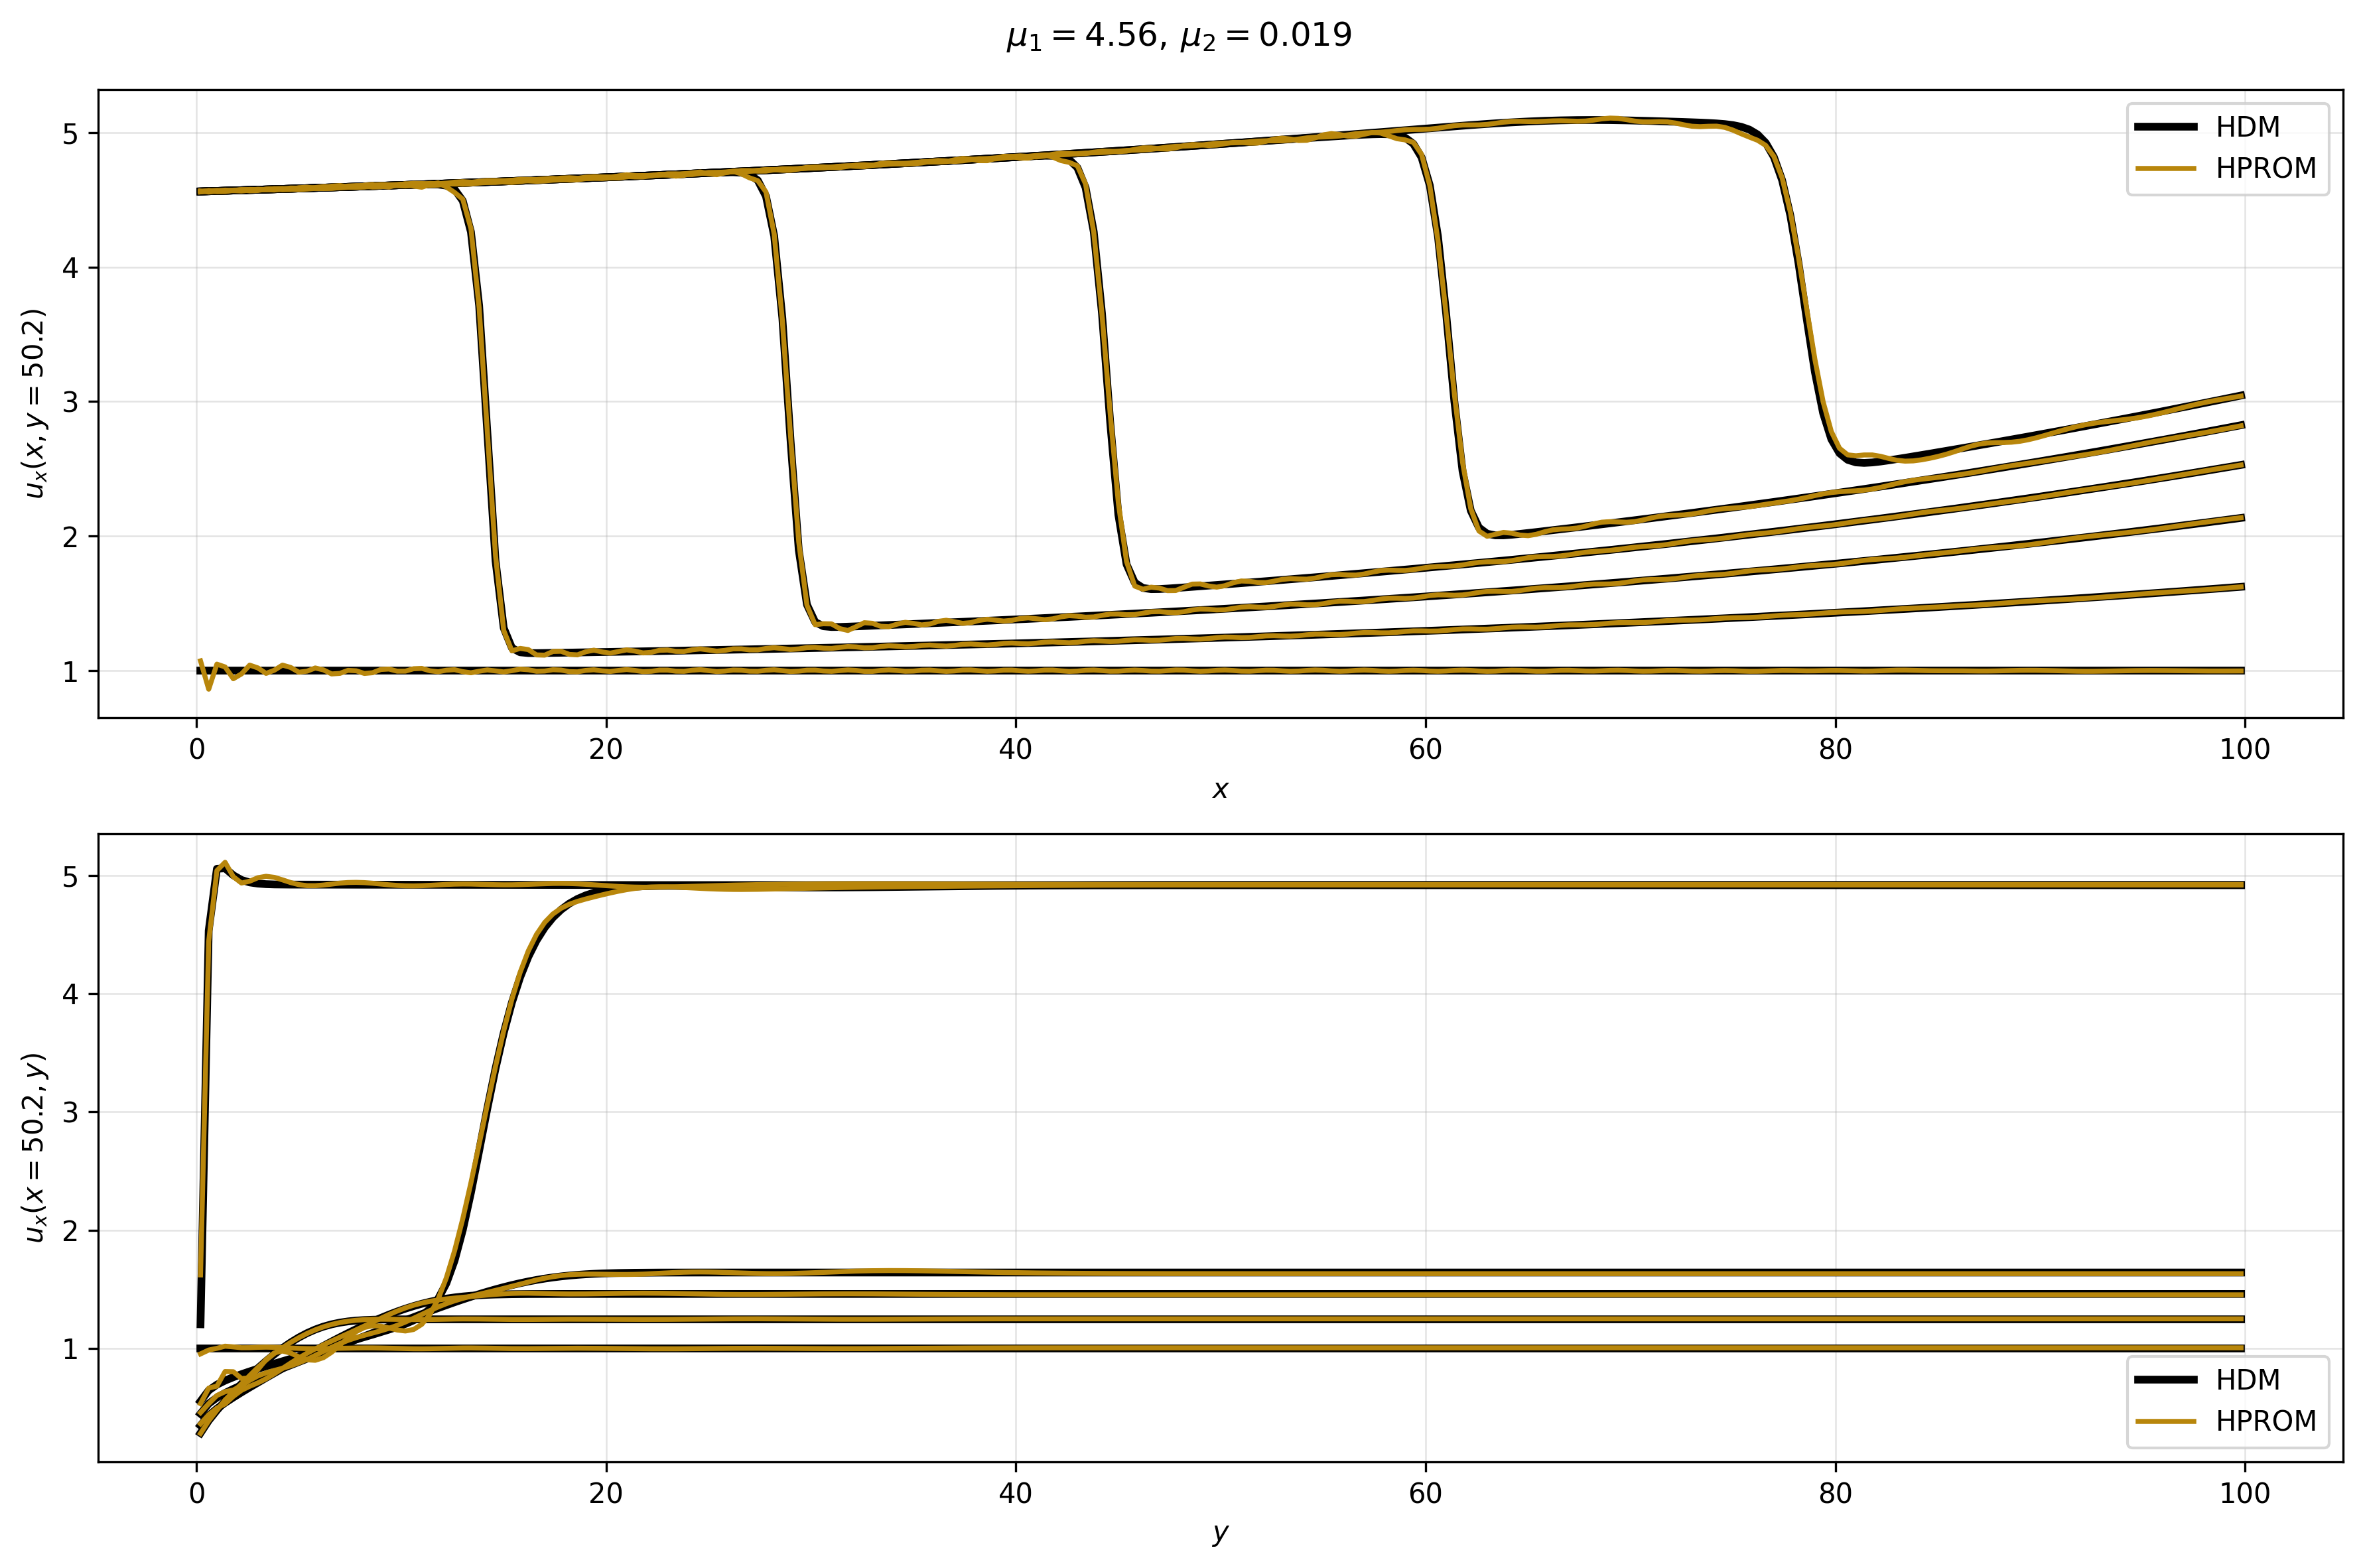
\includegraphics[width=0.80\textwidth]{Figures/hprom_vs_hdm.png}
\vspace{0.2em}

{\scriptsize $\mathbb{RE}_{2,\mathbf{u}}=0.450\%$ \quad $t=75.731$ s $(1.262$ min$)$ \quad speedup $=9.913\times$ \quad $N_e=5{,}722$}
\end{frame}

\begin{frame}{Local HPROM Solution ($250\times250$): $\boldsymbol{\mu}=(4.56,\,0.019)$}
\centering
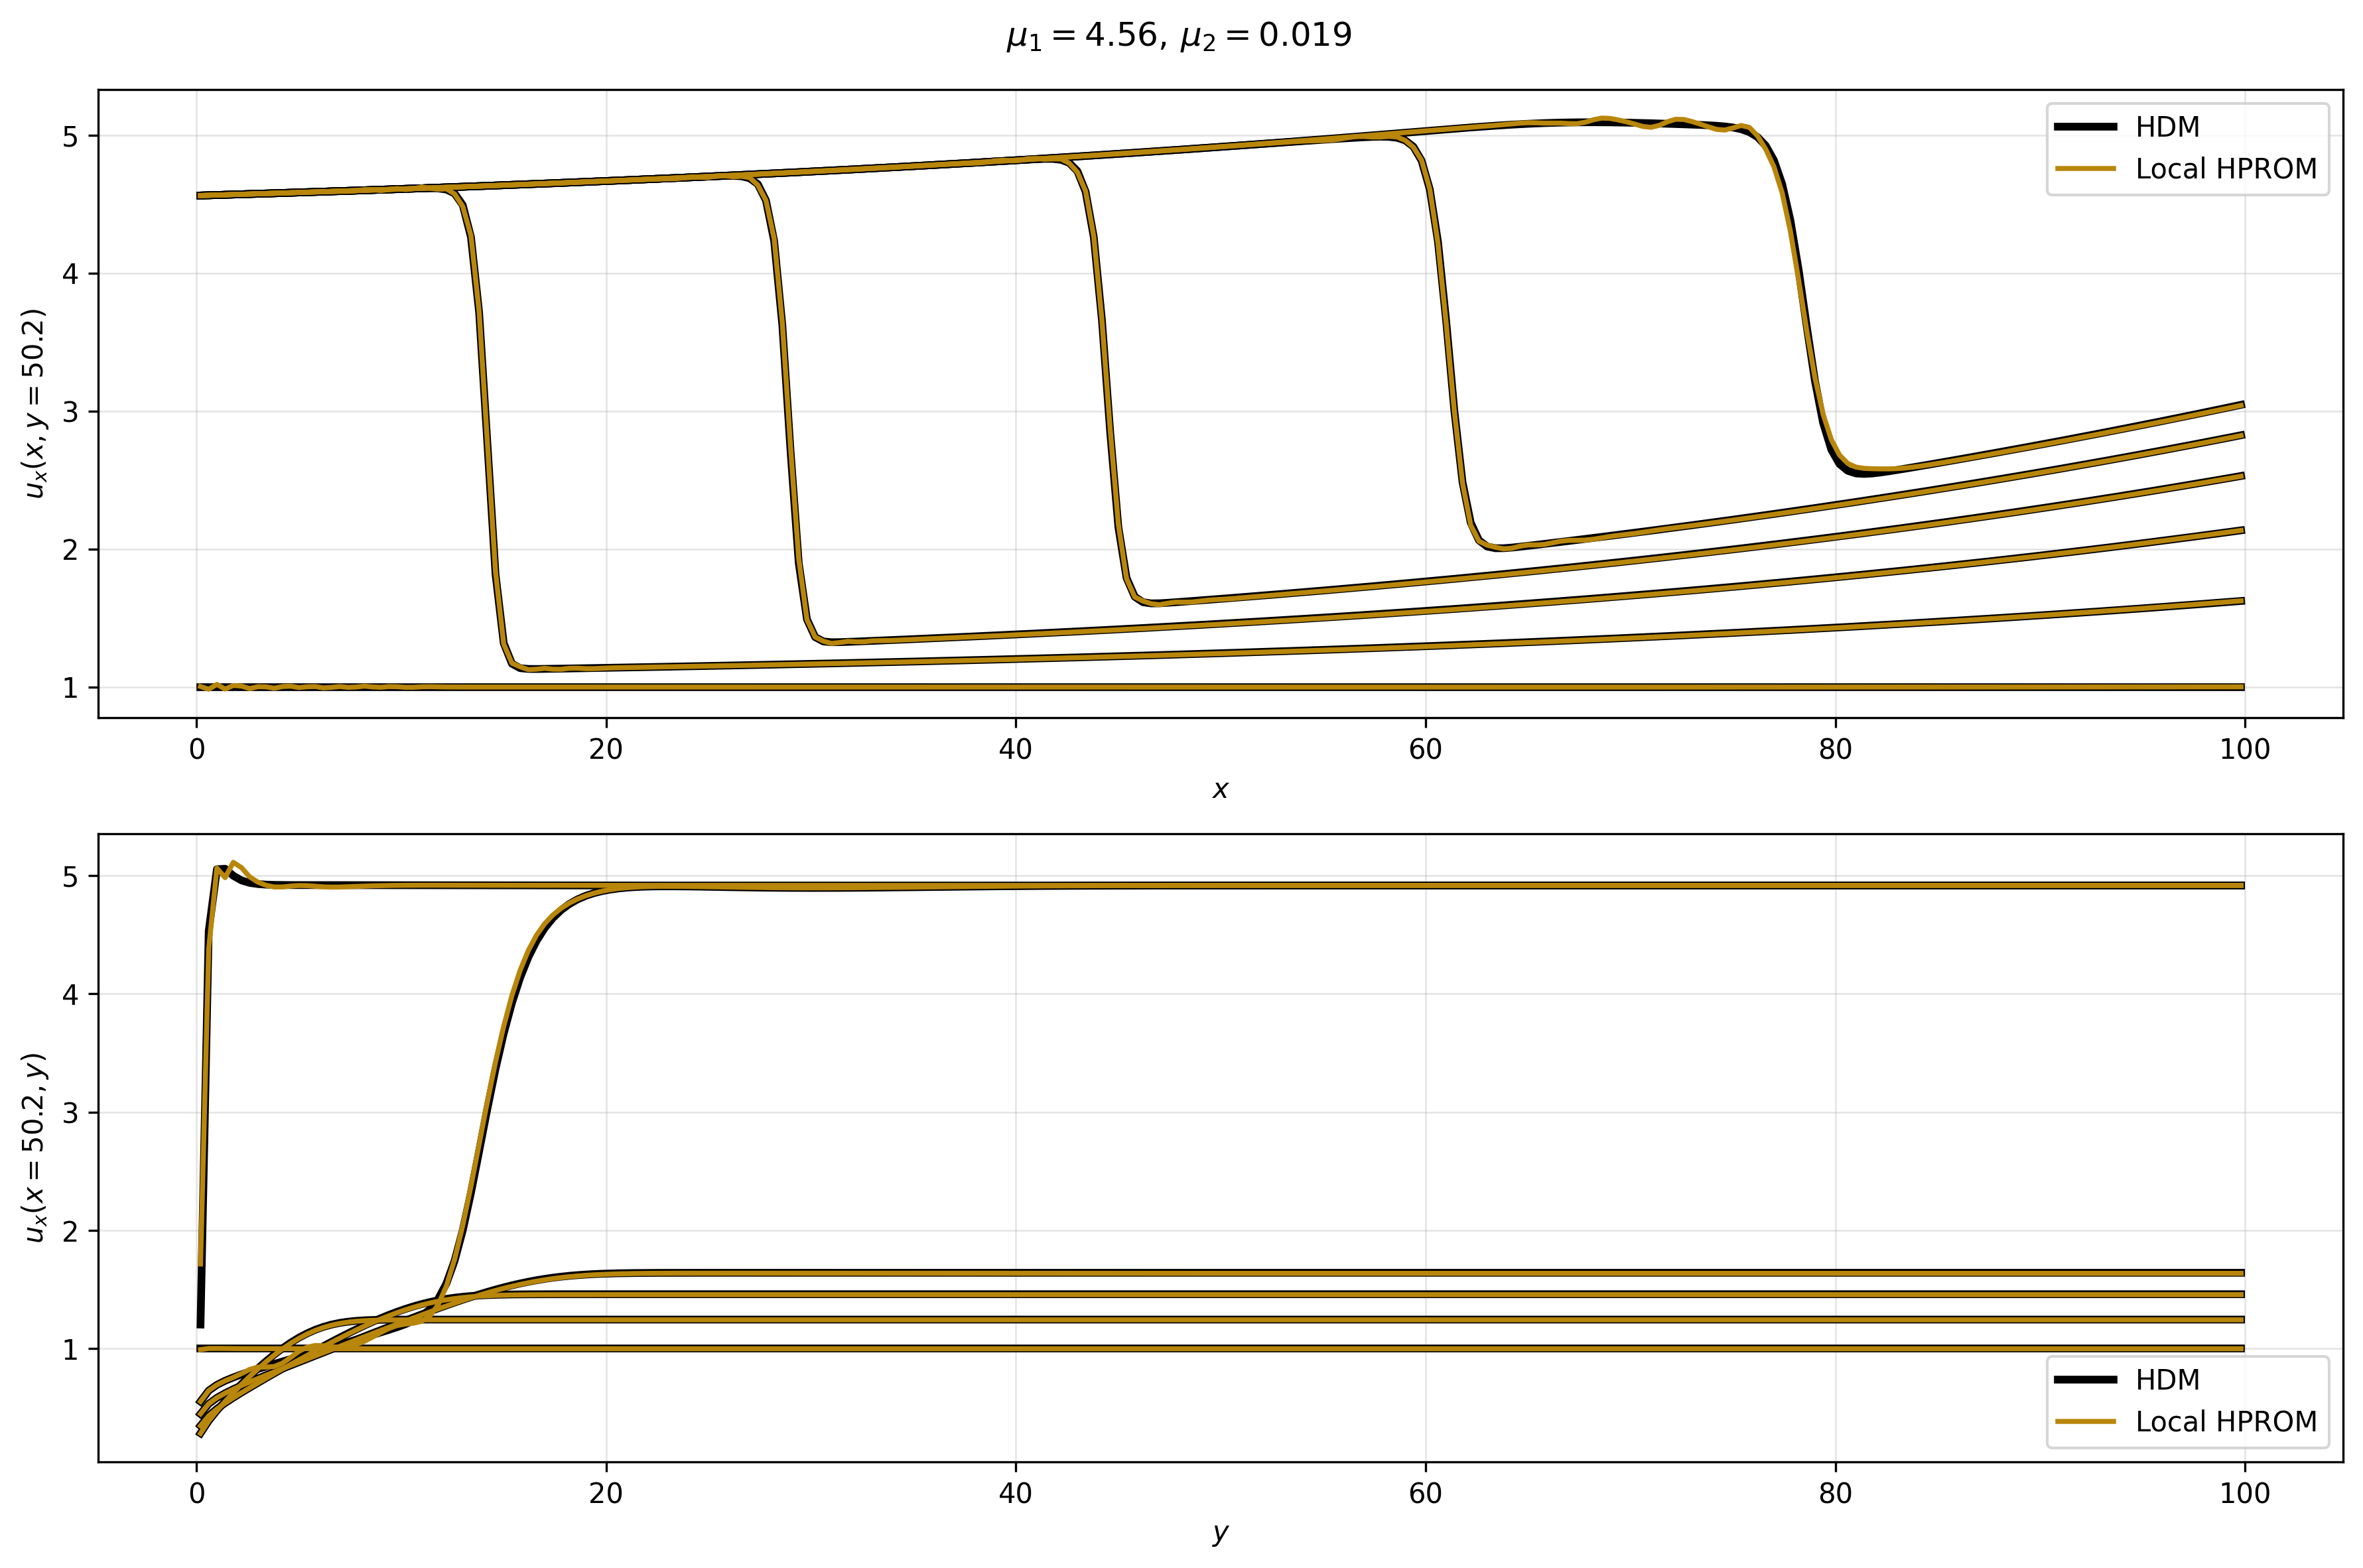
\includegraphics[width=0.80\textwidth]{Figures/local_hprom_vs_hdm.png}
\vspace{0.2em}

{\scriptsize $\mathbb{RE}_{2,\mathbf{u}}=0.228\%$ \quad $t=22.794$ s $(0.380$ min$)$ \quad speedup $=32.934\times$ \quad $N_e=2{,}951$}
\end{frame}

\begin{frame}{HQPROM Solution ($250\times250$): $\boldsymbol{\mu}=(4.56,\,0.019)$}
\centering
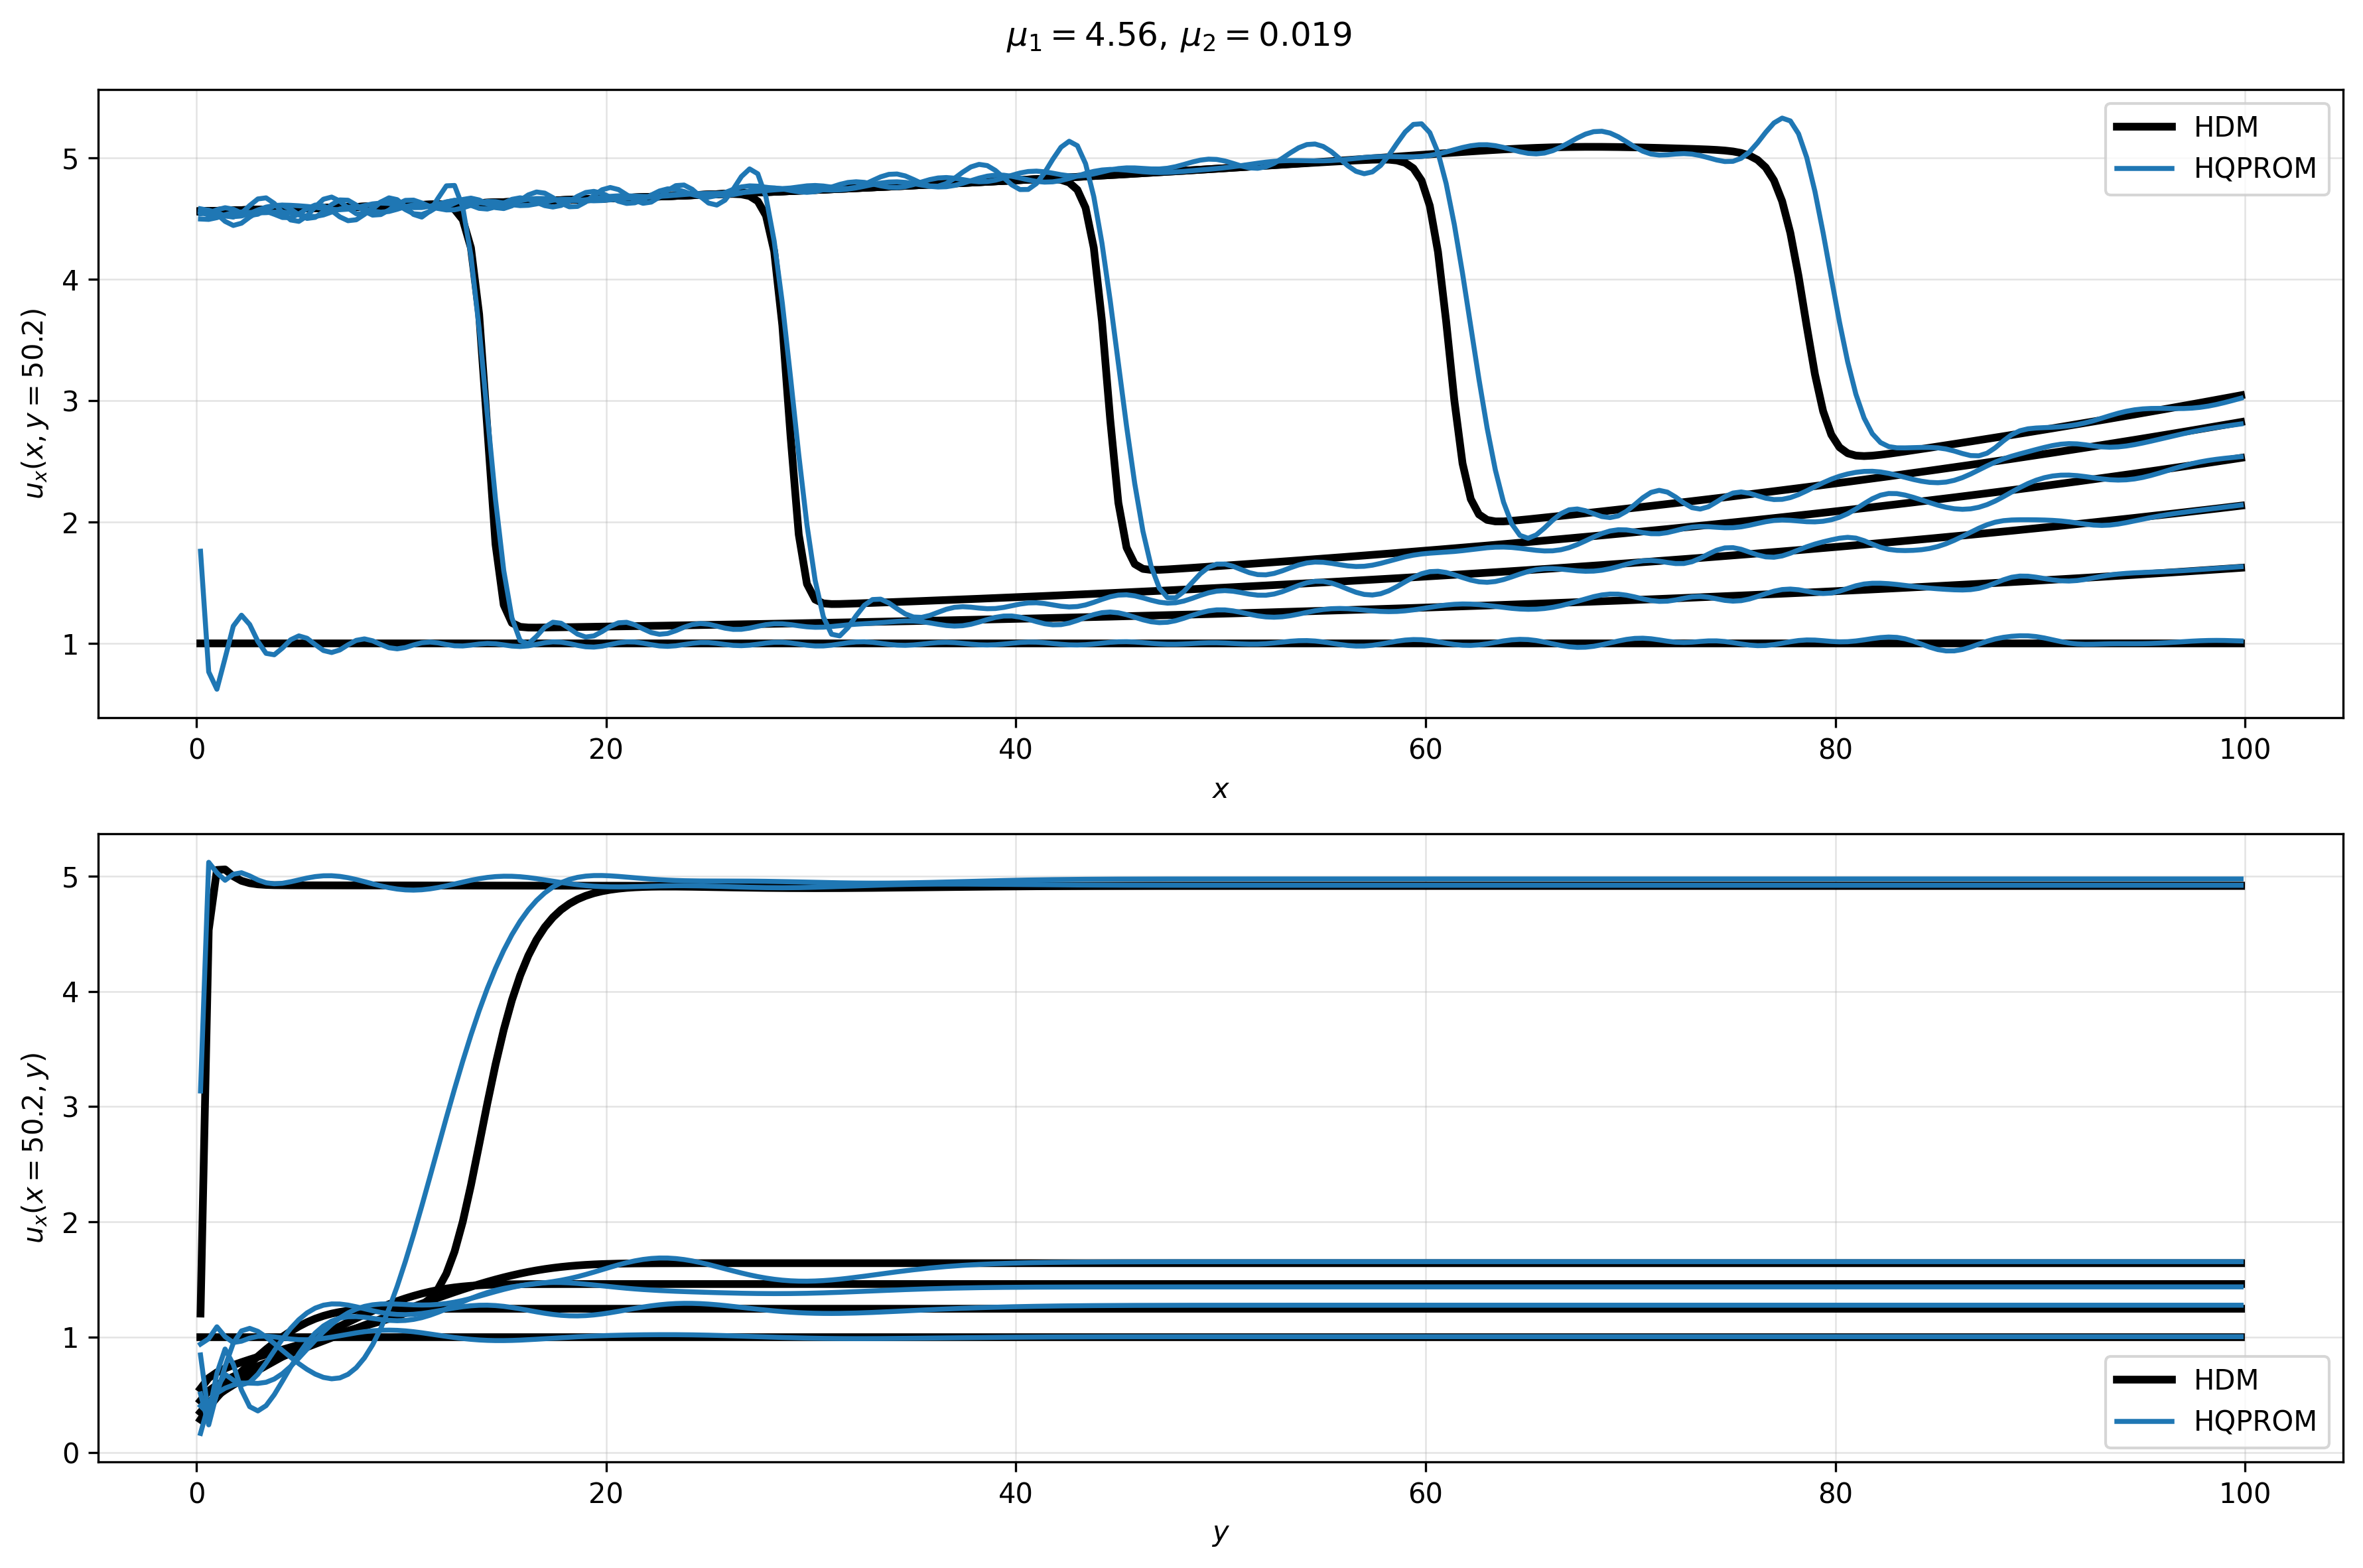
\includegraphics[width=0.80\textwidth]{Figures/hqprom_vs_hdm.png}
\vspace{0.2em}

{\scriptsize $\mathbb{RE}_{2,\mathbf{u}}=5.085\%$ \quad $t=21.734$ s $(0.362$ min$)$ \quad speedup $=34.541\times$ \quad $N_e=1{,}588$}
\end{frame}

\begin{frame}{Local HQPROM Solution ($250\times250$): $\boldsymbol{\mu}=(4.56,\,0.019)$}
\centering
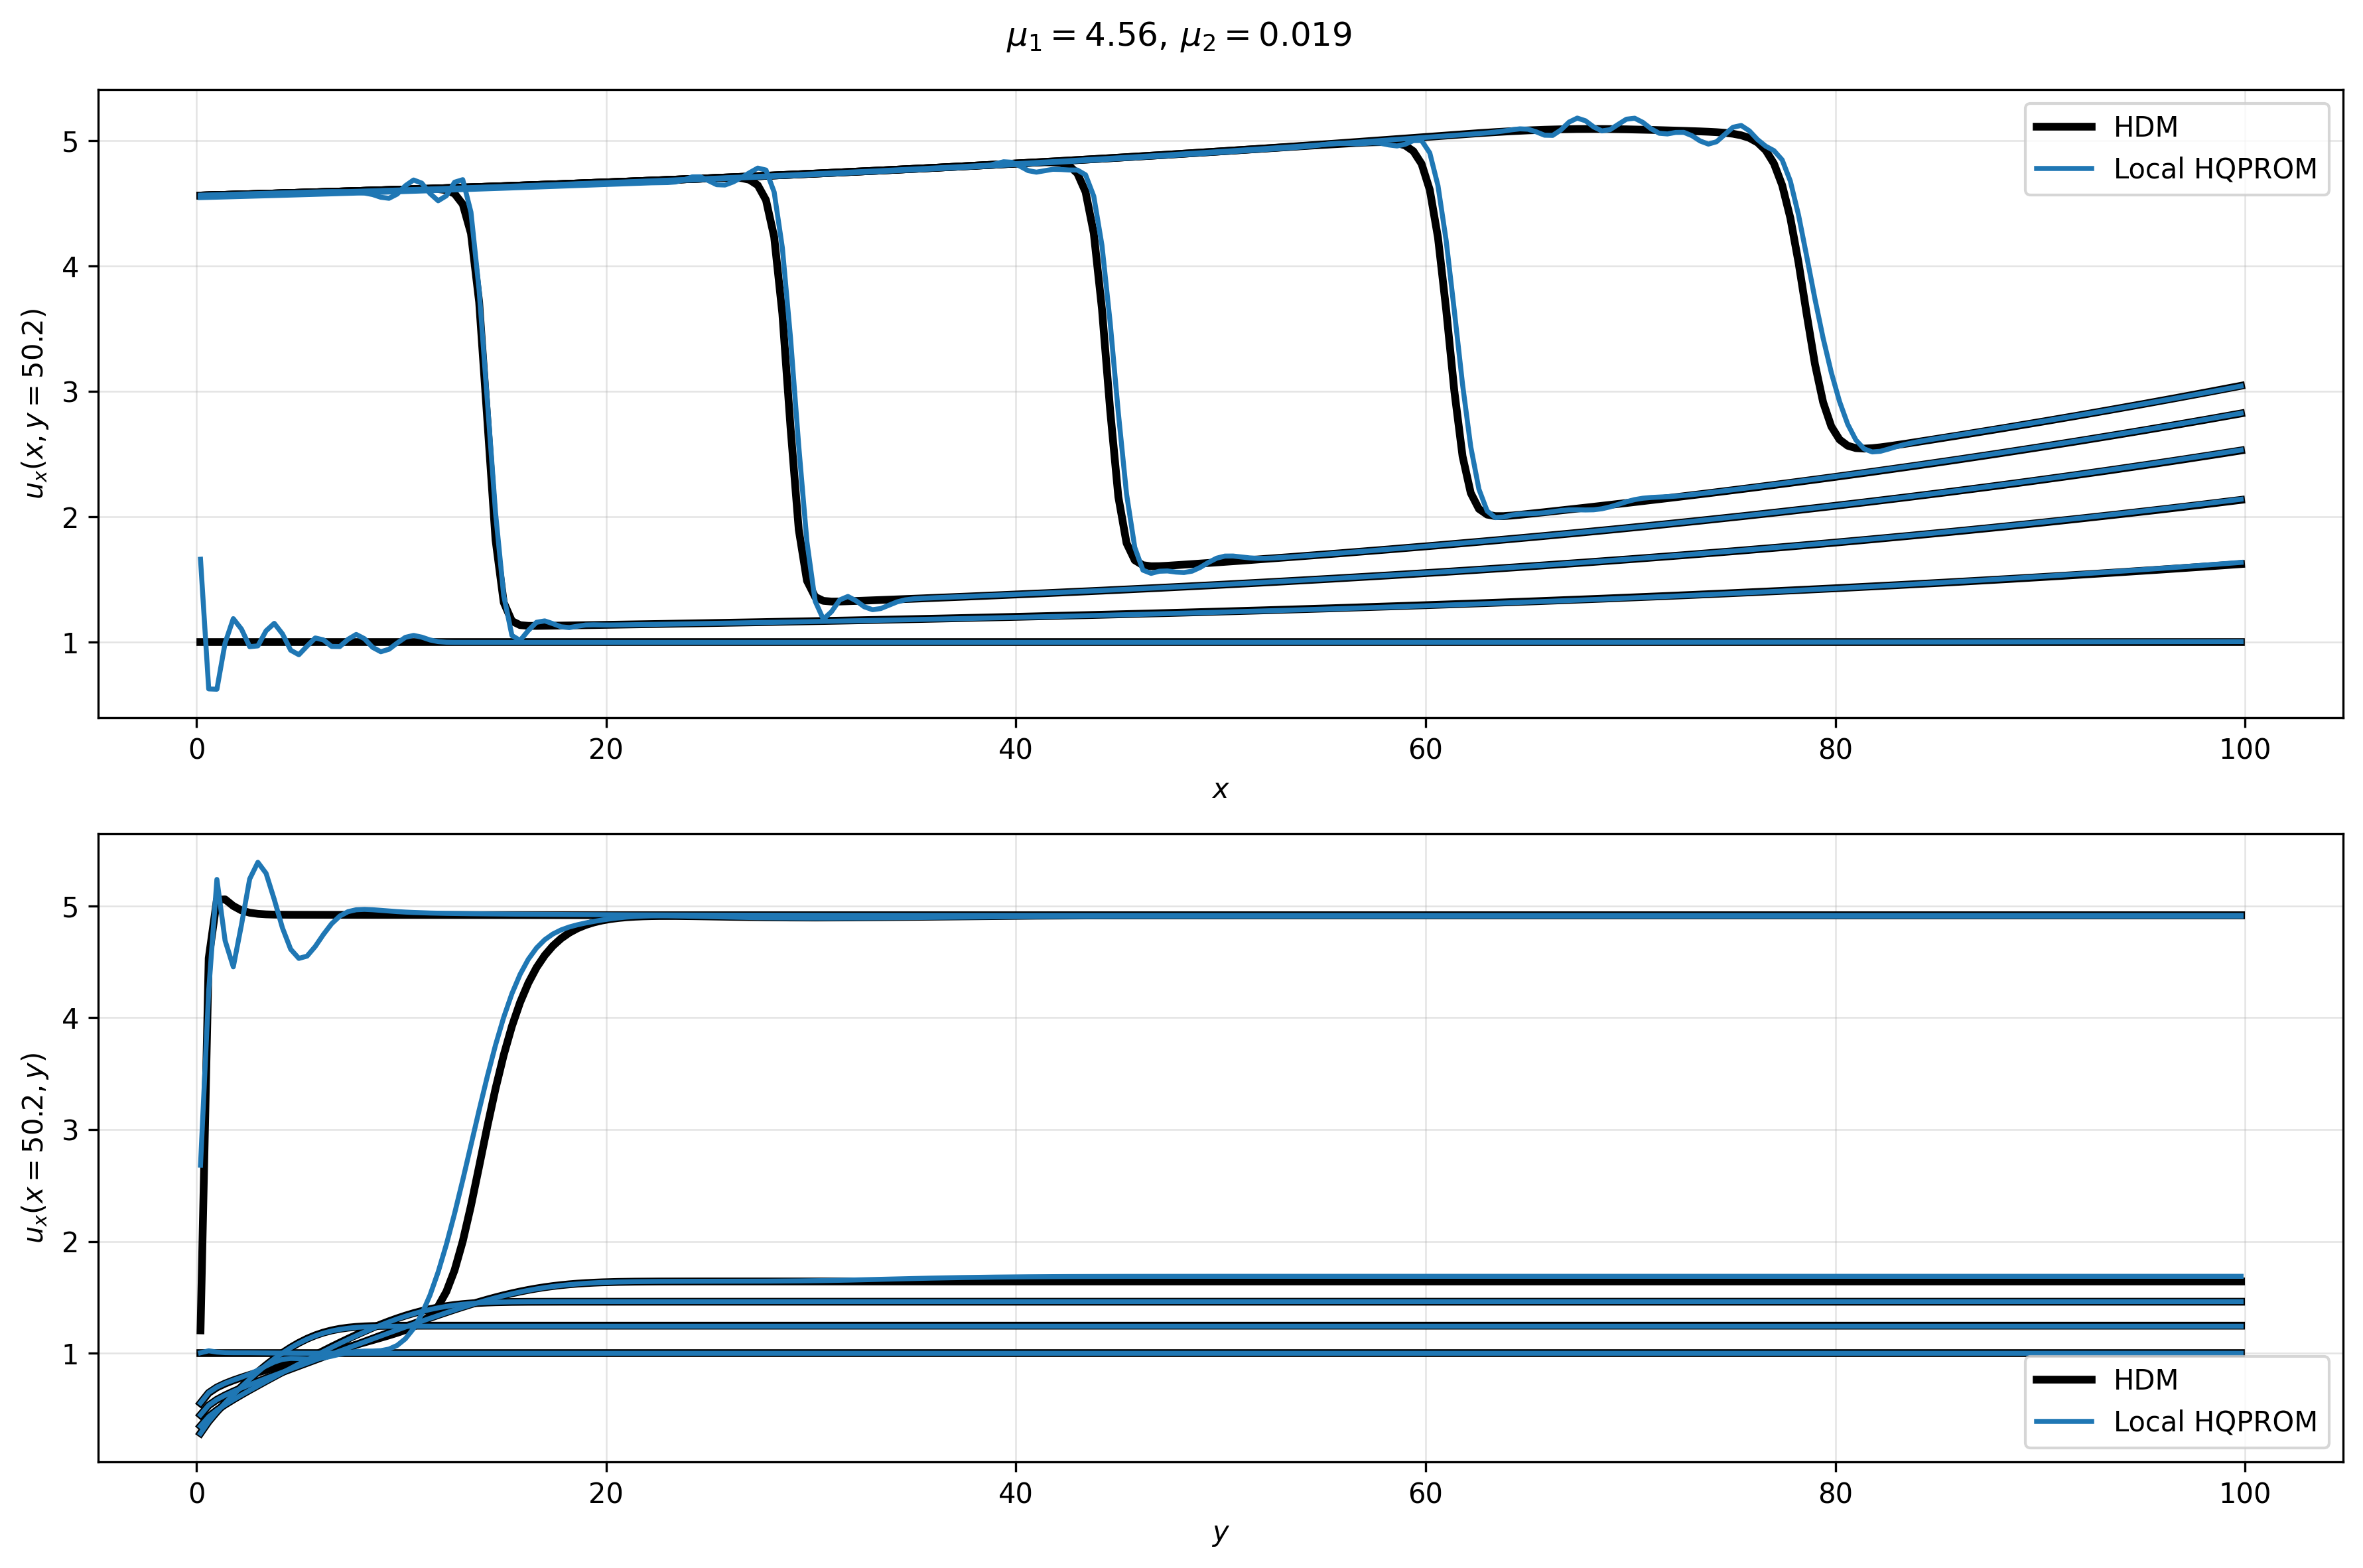
\includegraphics[width=0.80\textwidth]{Figures/local_hqprom_vs_hdm.png}
\vspace{0.2em}

{\scriptsize $\mathbb{RE}_{2,\mathbf{u}}=2.269\%$ \quad $t=15.463$ s $(0.258$ min$)$ \quad speedup $=48.550\times$ \quad $N_e=640$}
\end{frame}

\begin{frame}{HPROM-GPR Solution ($250\times250$): $\boldsymbol{\mu}=(4.56,\,0.019)$}
\centering
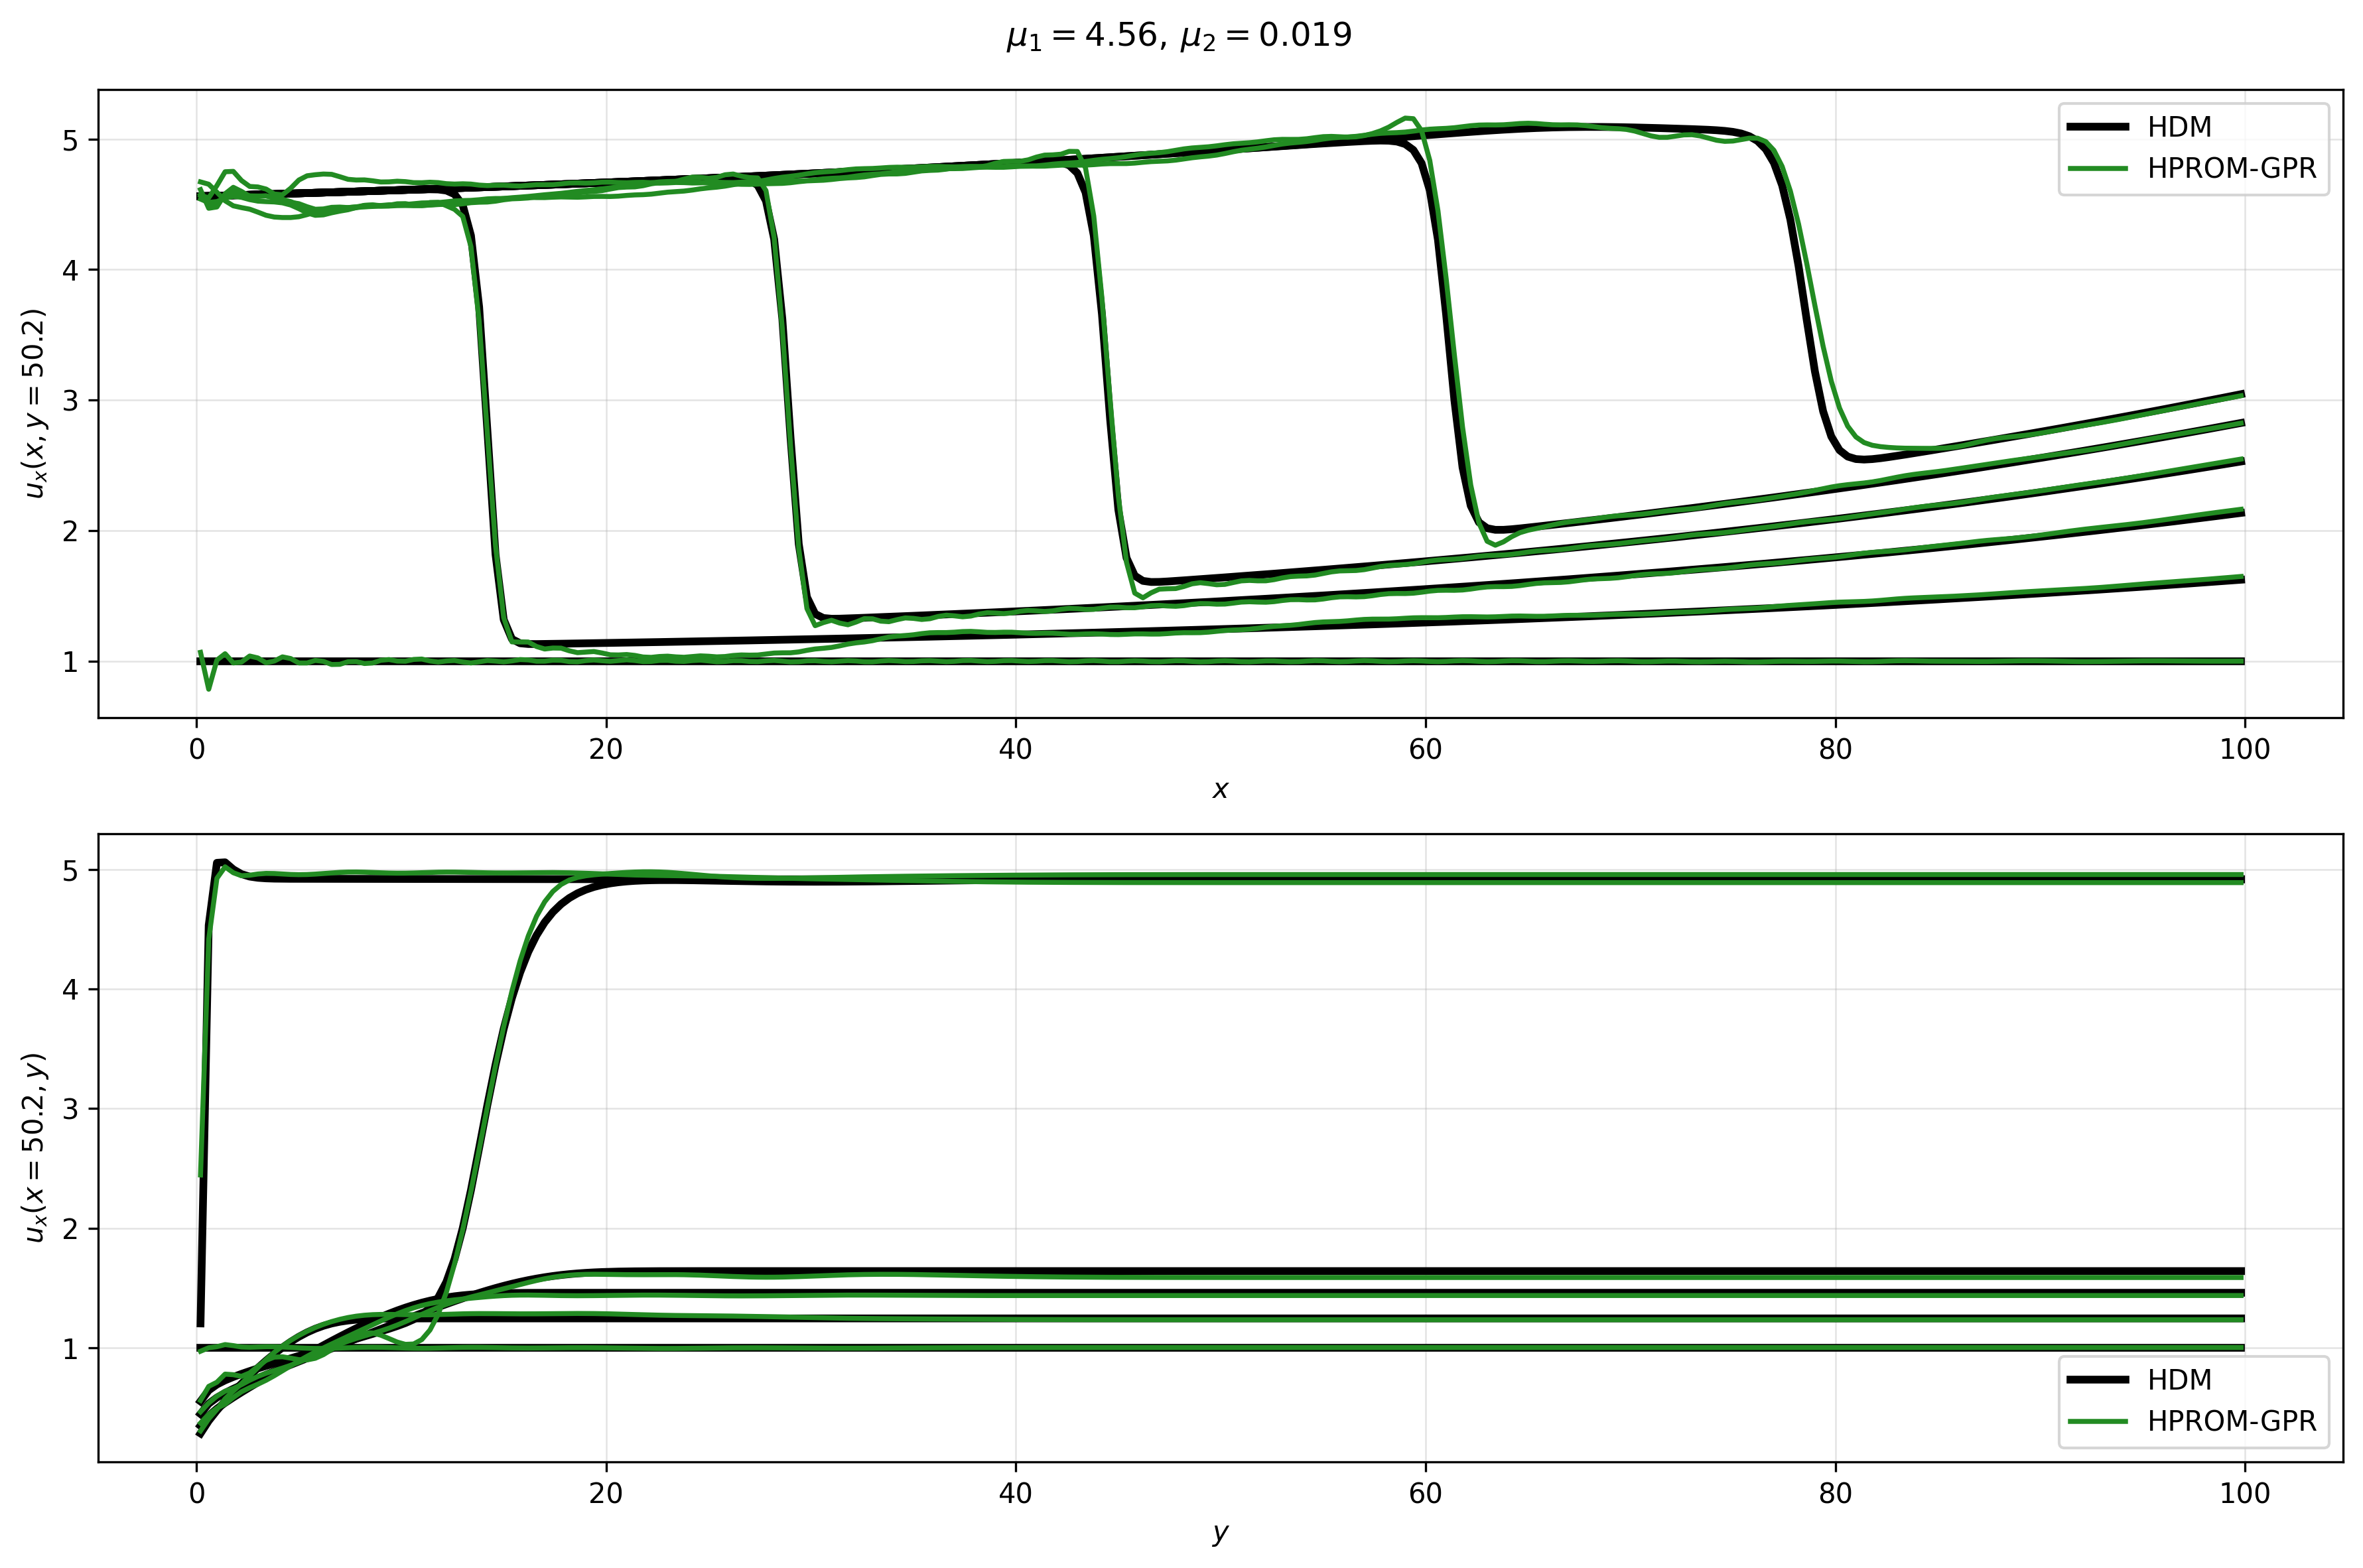
\includegraphics[width=0.80\textwidth]{Figures/hprom_gpr_vs_hdm.png}
\vspace{0.2em}

{\scriptsize $\mathbb{RE}_{2,\mathbf{u}}=2.103\%$ \quad $t=13.971$ s $(0.233$ min$)$ \quad speedup $=53.733\times$ \quad $N_e=901$}
\end{frame}

\begin{frame}{Local HPROM-GPR Solution ($250\times250$): $\boldsymbol{\mu}=(4.56,\,0.019)$}
\centering
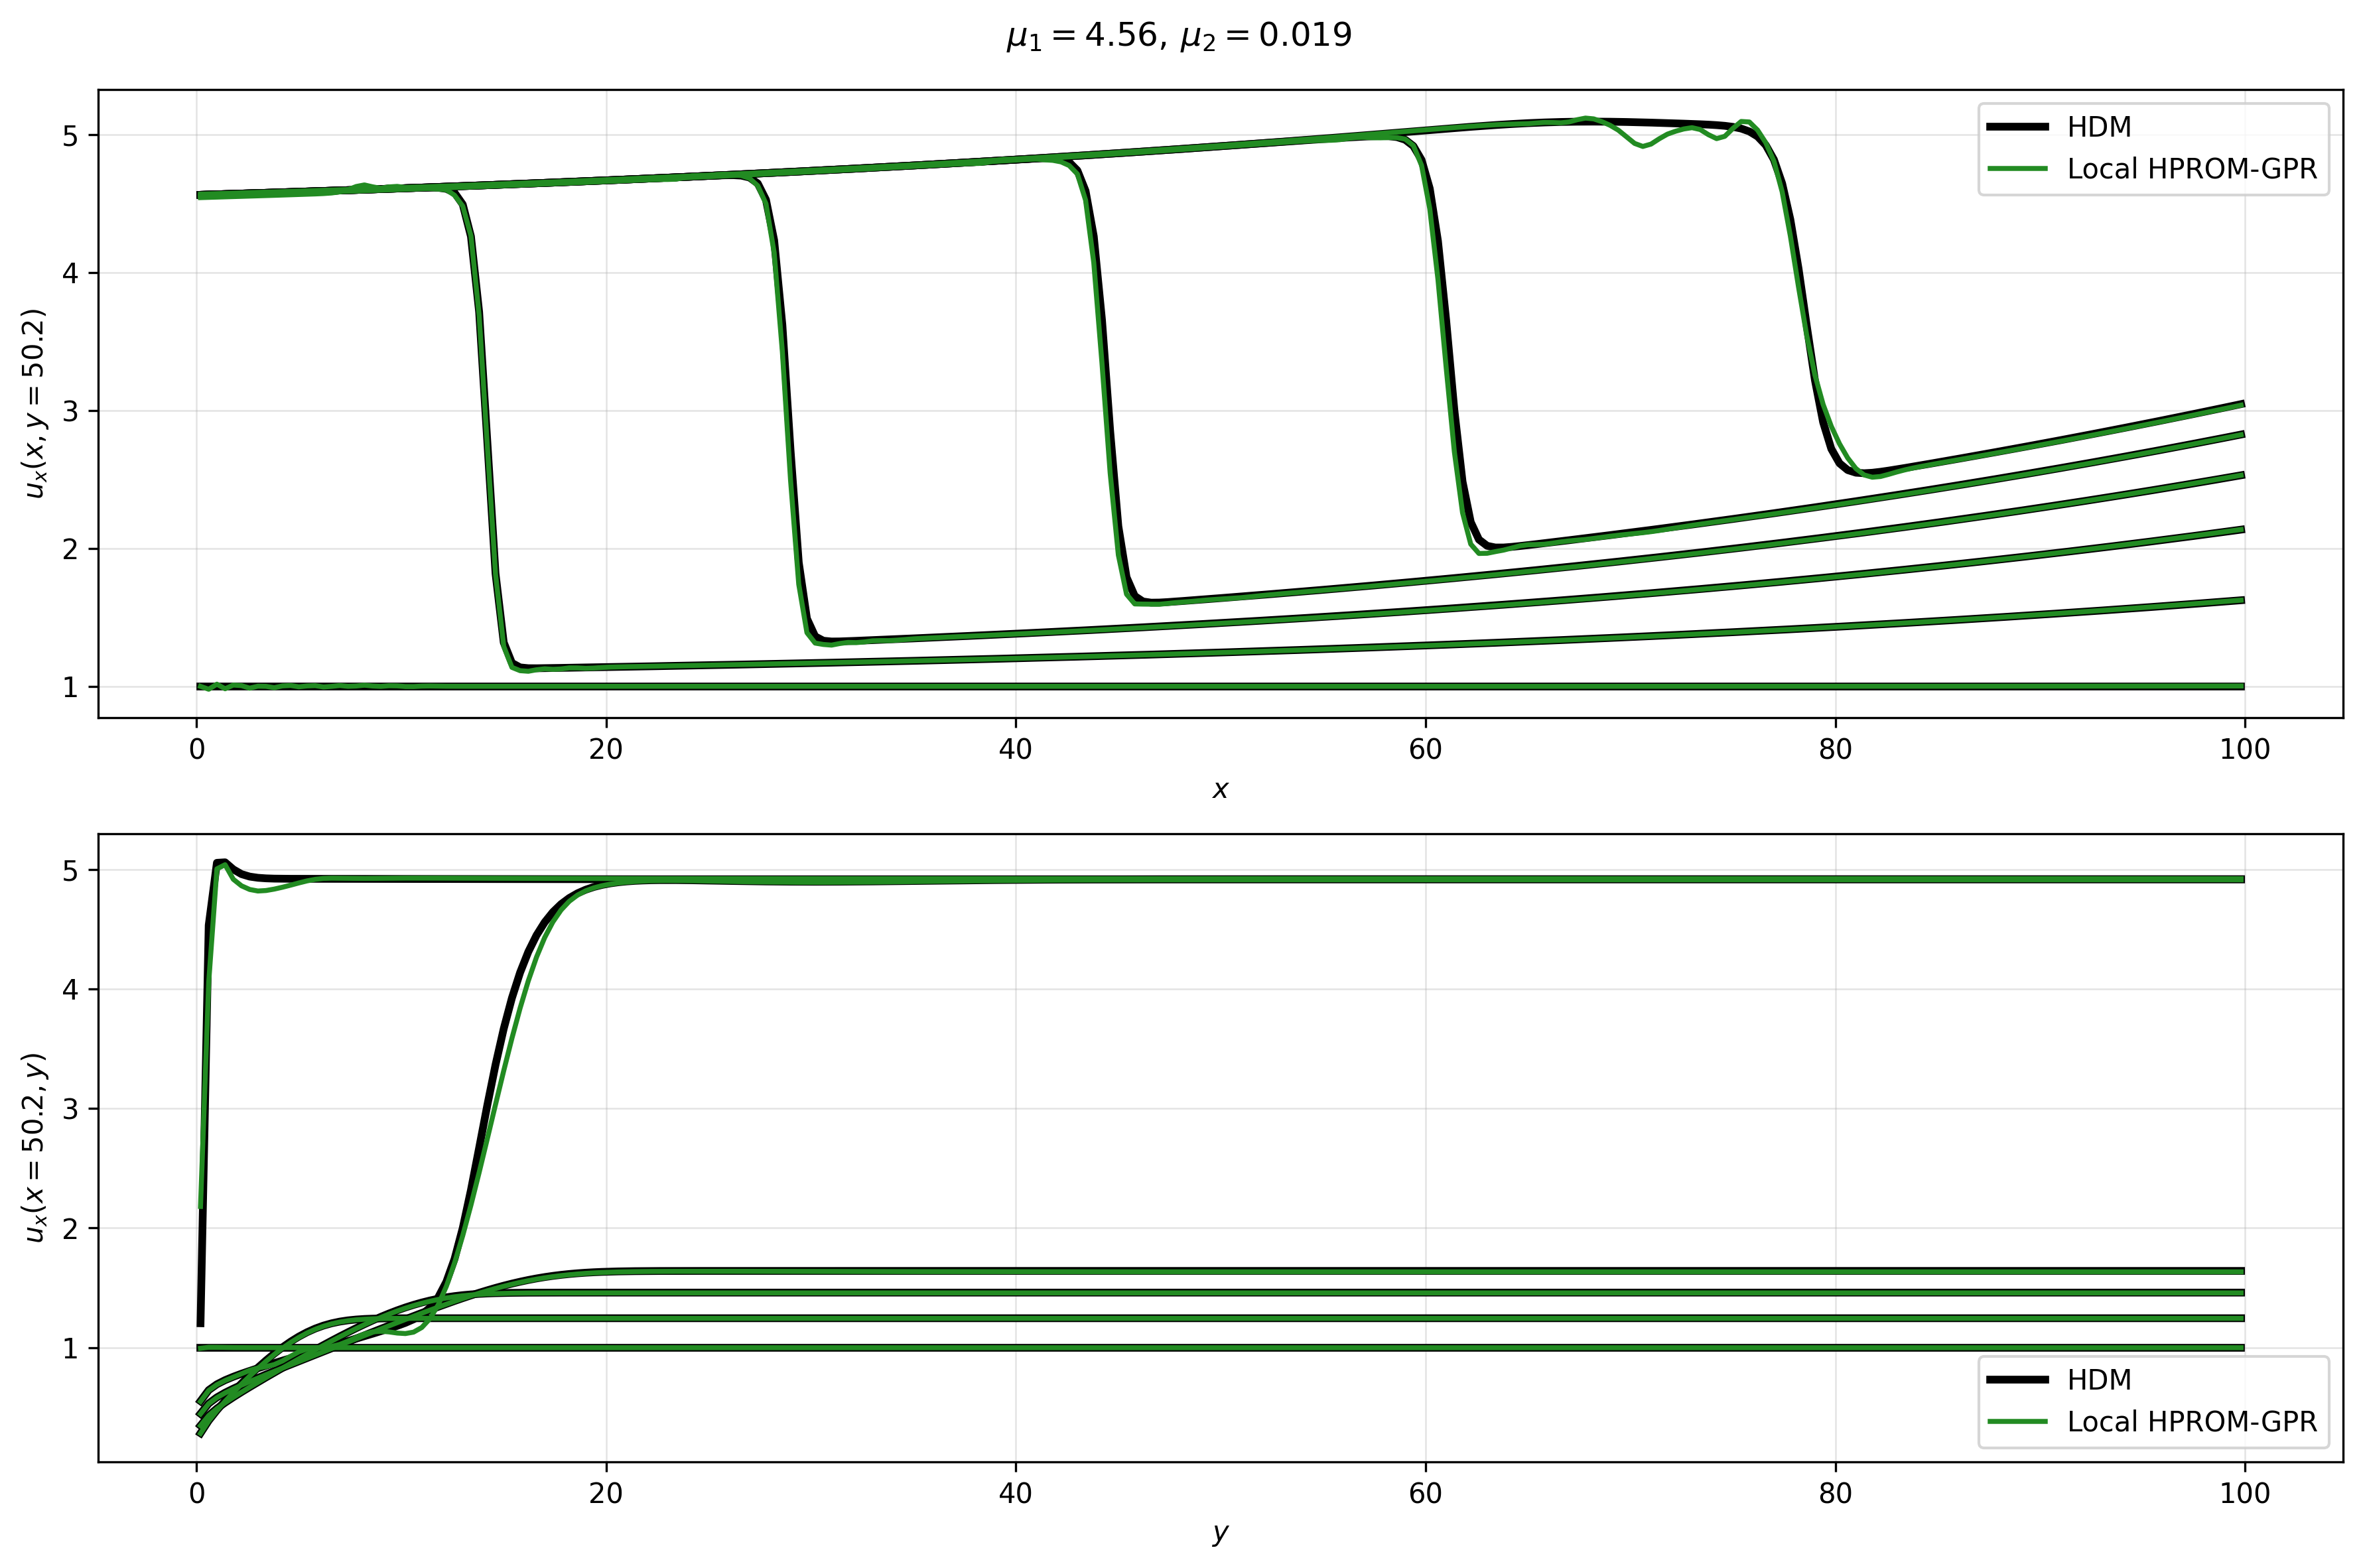
\includegraphics[width=0.80\textwidth]{Figures/local_hprom_gpr_vs_hdm.png}
\vspace{0.2em}

{\scriptsize $\mathbb{RE}_{2,\mathbf{u}}=1.008\%$ \quad $t=15.747$ s $(0.262$ min$)$ \quad speedup $=47.673\times$ \quad $N_e=451$}
\end{frame}

\begin{frame}{HPROM-POD-AE Solution ($250\times250$): $\boldsymbol{\mu}=(4.56,\,0.019)$}
\centering
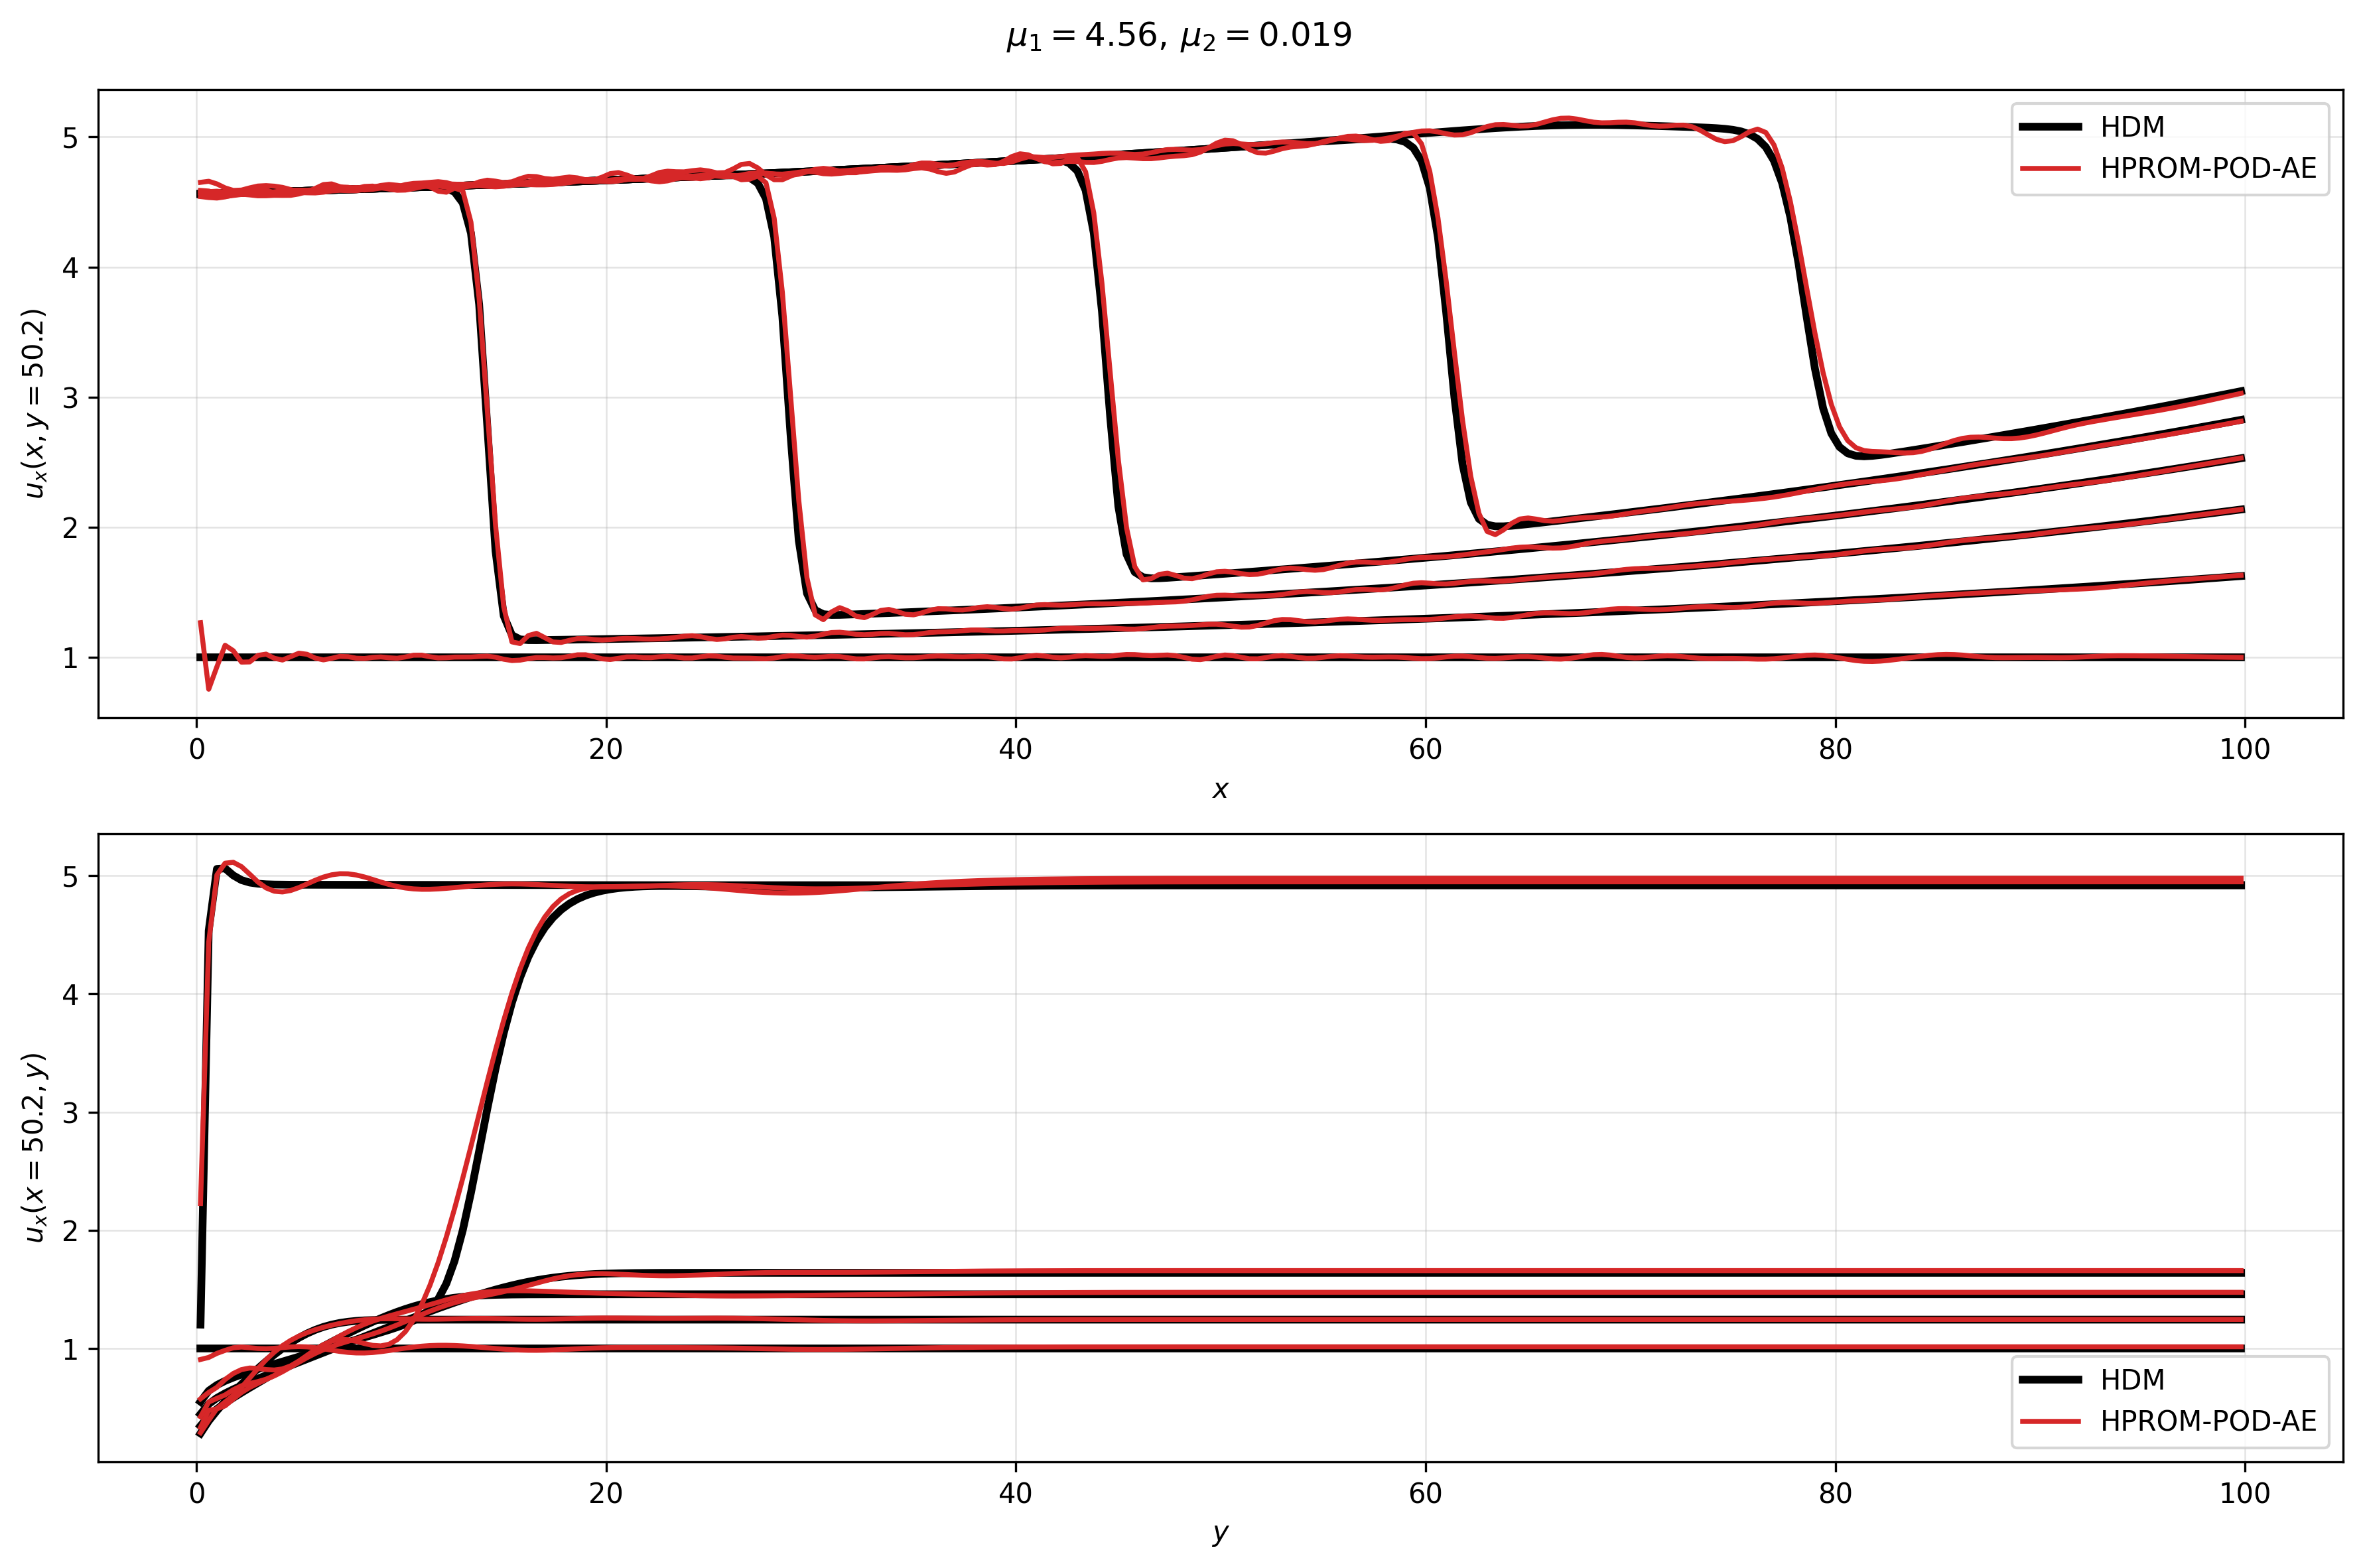
\includegraphics[width=0.80\textwidth]{Figures/hprom_dl_vs_hdm.png}
\vspace{0.2em}

{\scriptsize $\mathbb{RE}_{2,\mathbf{u}}=1.422\%$ \quad $t=12.451$ s $(0.208$ min$)$ \quad speedup $=60.291\times$ \quad $N_e=451$}
\end{frame}

\begin{frame}{Aero-F Implementation: Cylinder Case (Non-parametric)}
\small
Benchmark: 2D unsteady laminar viscous flow past a cylinder ($Re=100$), non-parametric setup.

\vspace{0.2em}
We report only HPROM-family results from the Aero-F workflow, using HDM as reference.

\vspace{0.2em}
\textbf{Reported metric}
\begin{itemize}
\item Drag error: relative $\ell_2$ error (\%) of drag $L_x$ over $t\in[0,150]$.
\end{itemize}

\vspace{0.2em}
{\scriptsize Aero-F ROM tutorial repository (non-parametric cylinder case):}

{\scriptsize \url{https://github.com/SADPR/aero-f_rom_turorial}}

{\scriptsize Runtimes were measured on a personal computer (not Sherlock), so wall-clock values are reference-only and may include parallel/background-load noise.}
\end{frame}

\begin{frame}{Aero-F Cylinder: HPROM Results Summary}
\tiny
\centering
\resizebox{\textwidth}{!}{%
\begin{tabular}{lrrrrrr}
\hline
\textbf{Computational model} & $n$ ($N$ for HDM) & $\bar{n}$ & $N_e$ & $\mathbb{RE}_{2,L_x}$ (\%) & Wall-clock time (min) & Speedup \\
\hline
HDM & 490\,700 & -- & 98\,140 & -- & 218.622 & -- \\
\addlinespace[0.35em]
HPROM & 35 & -- & 336 & 0.117 & 0.315 & 694.040 \\
HQPROM & 10 & -- & 165 & 0.356 & 0.148 & 1\,472.204 \\
HPROM-ANN & 5 & 30 & 93 & 0.159 & 0.092 & 2\,367.751 \\
HPROM-RBF & 5 & 30 & 87 & 0.167 & 0.064 & 3\,407.101 \\
HPROM-GPR & 5 & 30 & 81 & 0.134 & 0.058 & 3\,769.351 \\
\addlinespace[0.35em]
Local-HPROM ($N_c=3$) & 14--35 & -- & 253 & 0.062 & 0.179 & 1\,223.632 \\
Local-HQPROM ($N_c=3$) & 7--10 & -- & 157 & 0.730 & 0.106 & 2\,068.981 \\
Local-HPROM-ANN ($N_c=3$) & 3 & 11--32 & 56 & 0.382 & 0.066 & 3\,329.274 \\
Local-HPROM-RBF ($N_c=3$) & 3 & 11--32 & 73 & 0.145 & 0.036 & 6\,044.857 \\
Local-HPROM-GPR ($N_c=3$) & 3 & 11--32 & 53 & 0.371 & 0.029 & 7\,670.959 \\
\hline
\end{tabular}}
\vspace{0.2em}

{\tiny Drag error: relative \(\ell_2\) (\%) of \(L_x\) on \(t\in[0,150]\). Speedup uses \(t_{\mathrm{HDM}}=13{,}117.340\) s.}
{\tiny Global ANN/RBF/GPR use \(n=5\), \(\bar n=30\). Local ANN/RBF/GPR use \(n=3\), \(\bar n\in[11,32]\).}
\end{frame}

\begin{frame}{Aero-F Cylinder: HPROM vs HDM (Drag $L_x$)}
\centering
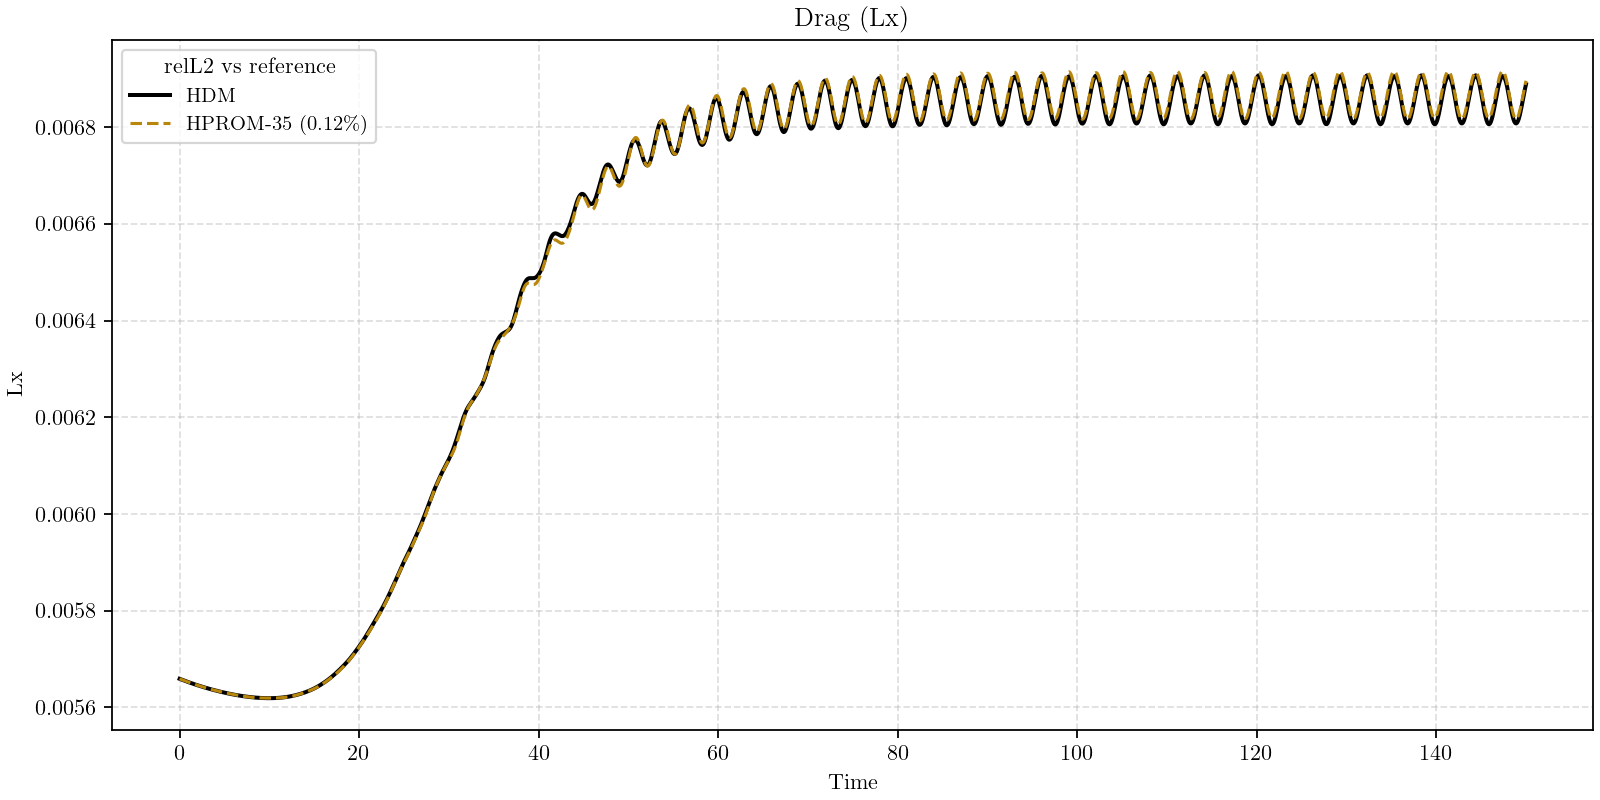
\includegraphics[width=0.92\textwidth]{Figures_AeroF/hprom_35_vs_hdm_drag_lx.png}
\end{frame}

\begin{frame}{Aero-F Cylinder: Local-HPROM ($N_c=3$) vs HDM (Drag $L_x$)}
\centering
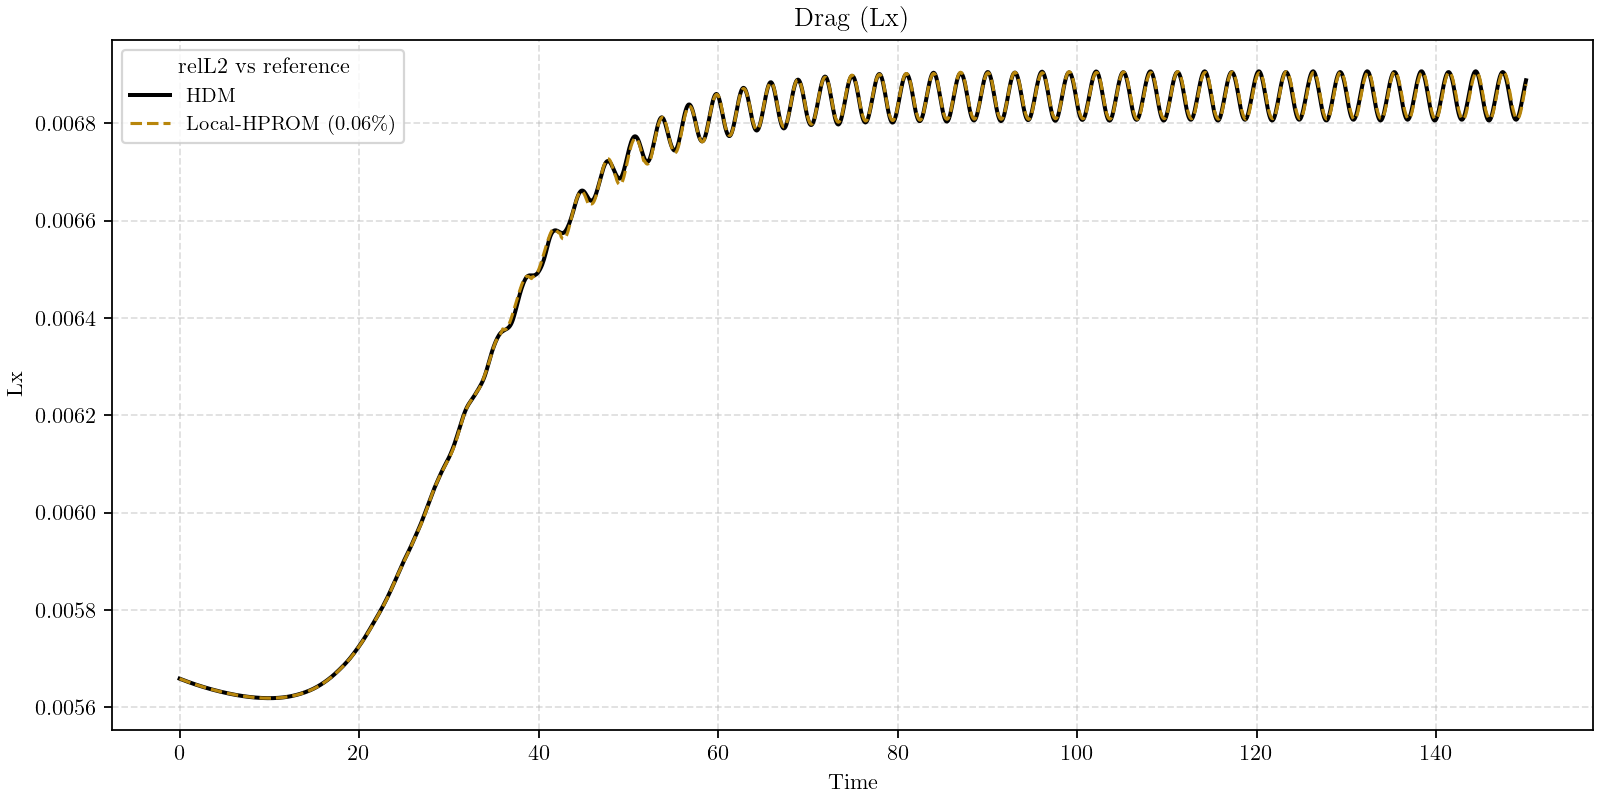
\includegraphics[width=0.92\textwidth]{Figures_AeroF/hprom_local_vs_hdm_drag_lx.png}
\end{frame}

\begin{frame}{Aero-F Cylinder: HQPROM vs HDM (Drag $L_x$)}
\centering
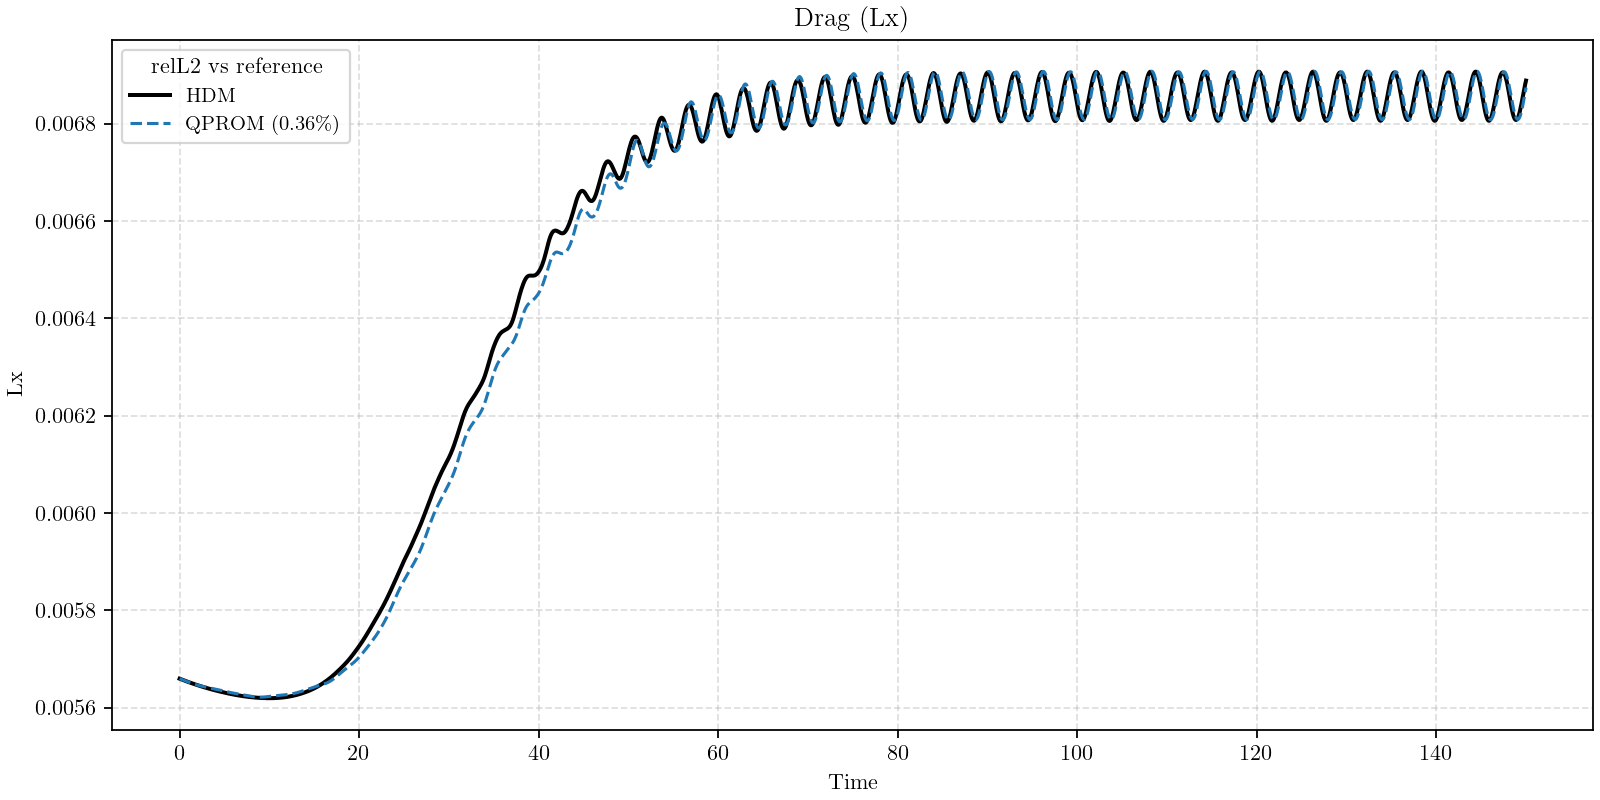
\includegraphics[width=0.92\textwidth]{Figures_AeroF/hprom_quad_vs_hdm_drag_lx.png}
\end{frame}

\begin{frame}{Aero-F Cylinder: Local-HQPROM ($N_c=3$) vs HDM (Drag $L_x$)}
\centering
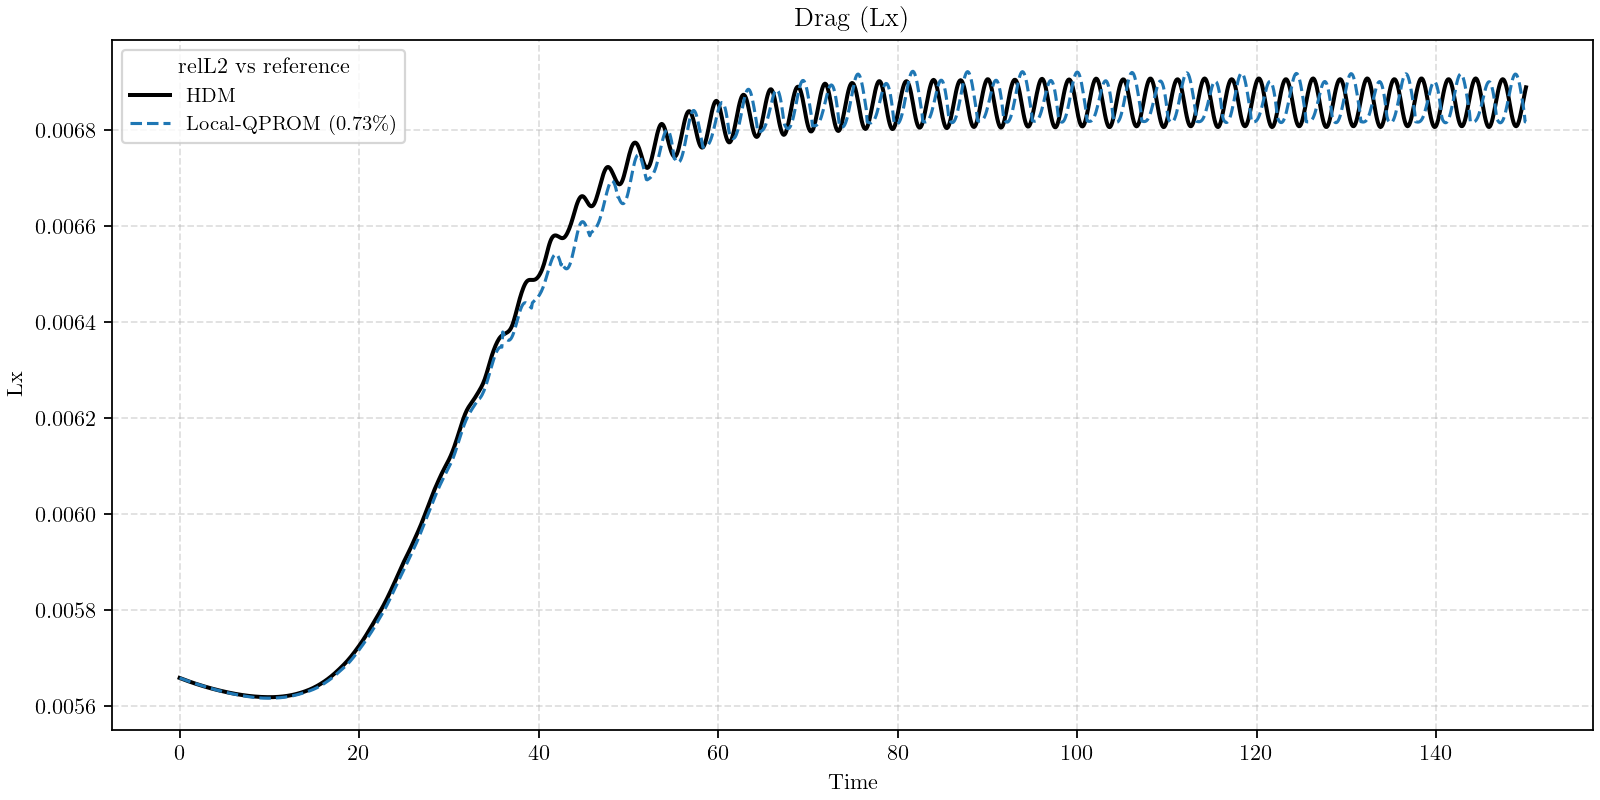
\includegraphics[width=0.92\textwidth]{Figures_AeroF/hprom_local_quad_vs_hdm_drag_lx.png}
\end{frame}

\begin{frame}{Aero-F Cylinder: HPROM-ANN vs HDM (Drag $L_x$)}
\centering
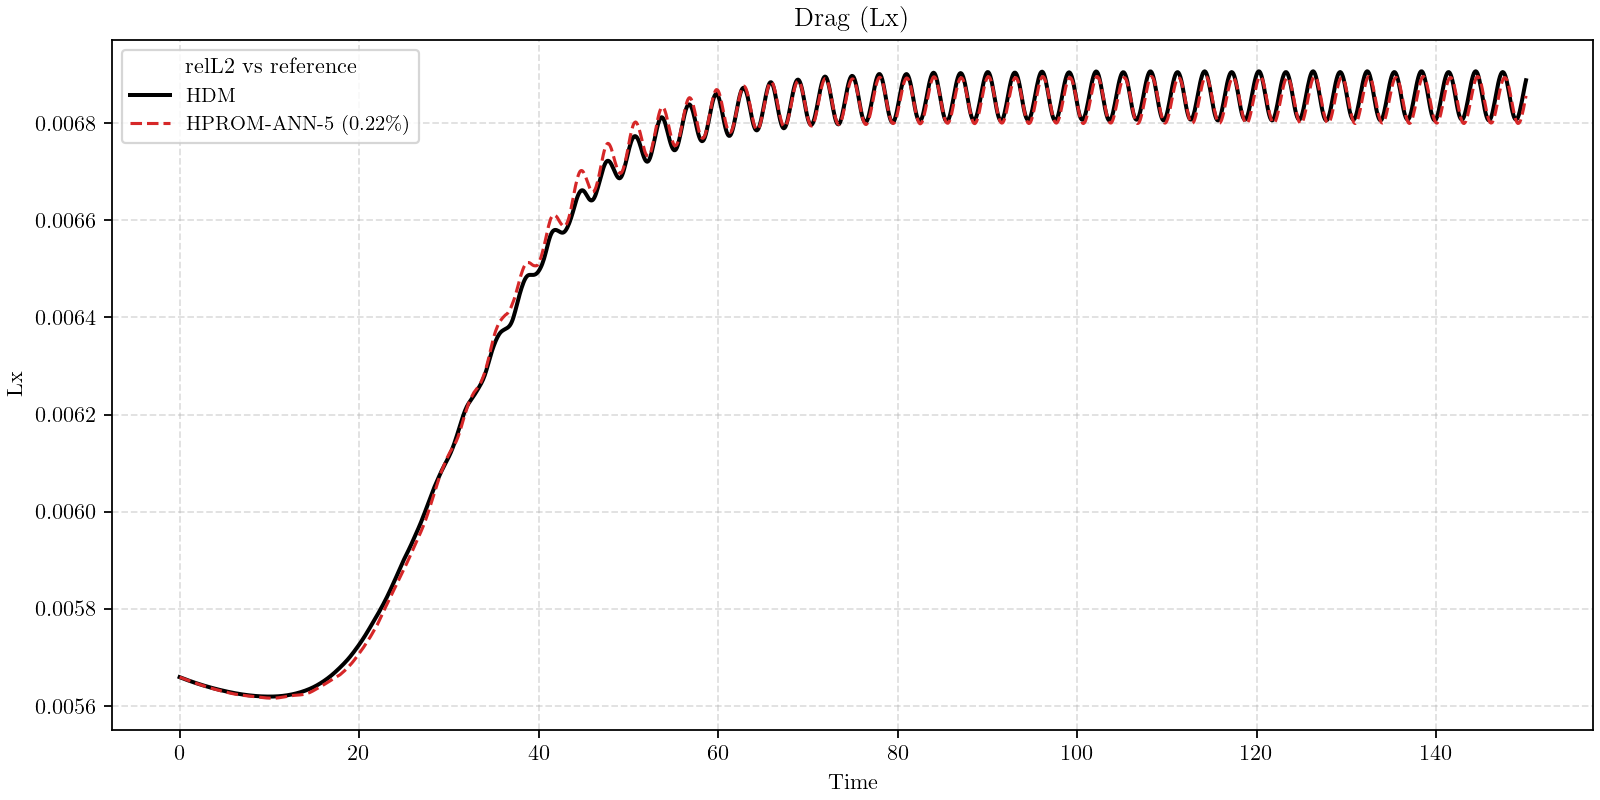
\includegraphics[width=0.92\textwidth]{Figures_AeroF/hprom_ann_5_vs_hdm_drag_lx.png}
\end{frame}

\begin{frame}{Aero-F Cylinder: Local-HPROM-ANN ($N_c=3$) vs HDM (Drag $L_x$)}
\centering
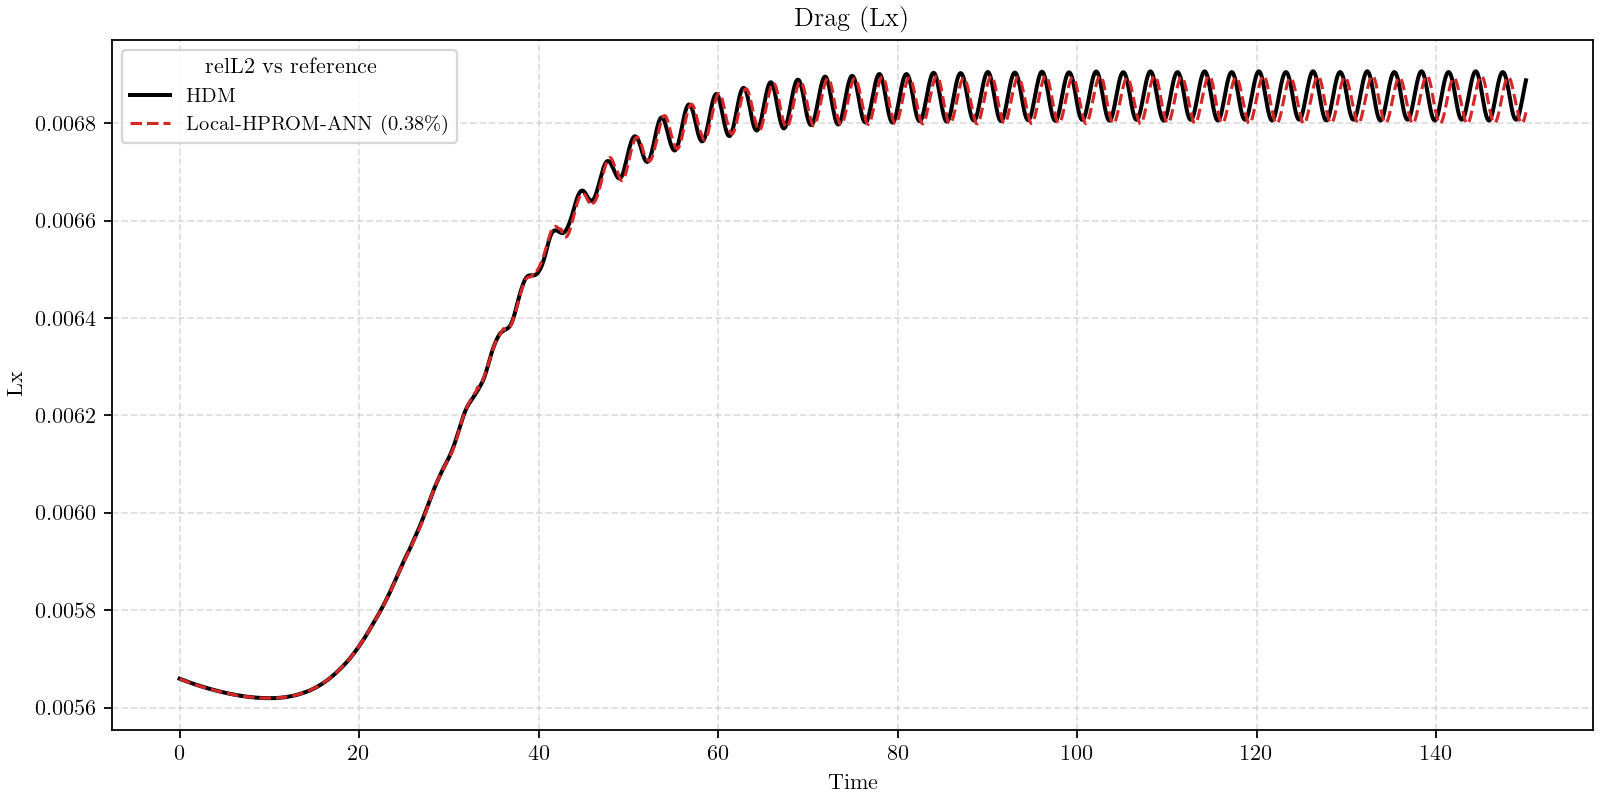
\includegraphics[width=0.92\textwidth]{Figures_AeroF/hprom_local_ann_vs_hdm_drag_lx.png}
\end{frame}

\begin{frame}{Aero-F Cylinder: HPROM-RBF vs HDM (Drag $L_x$)}
\centering
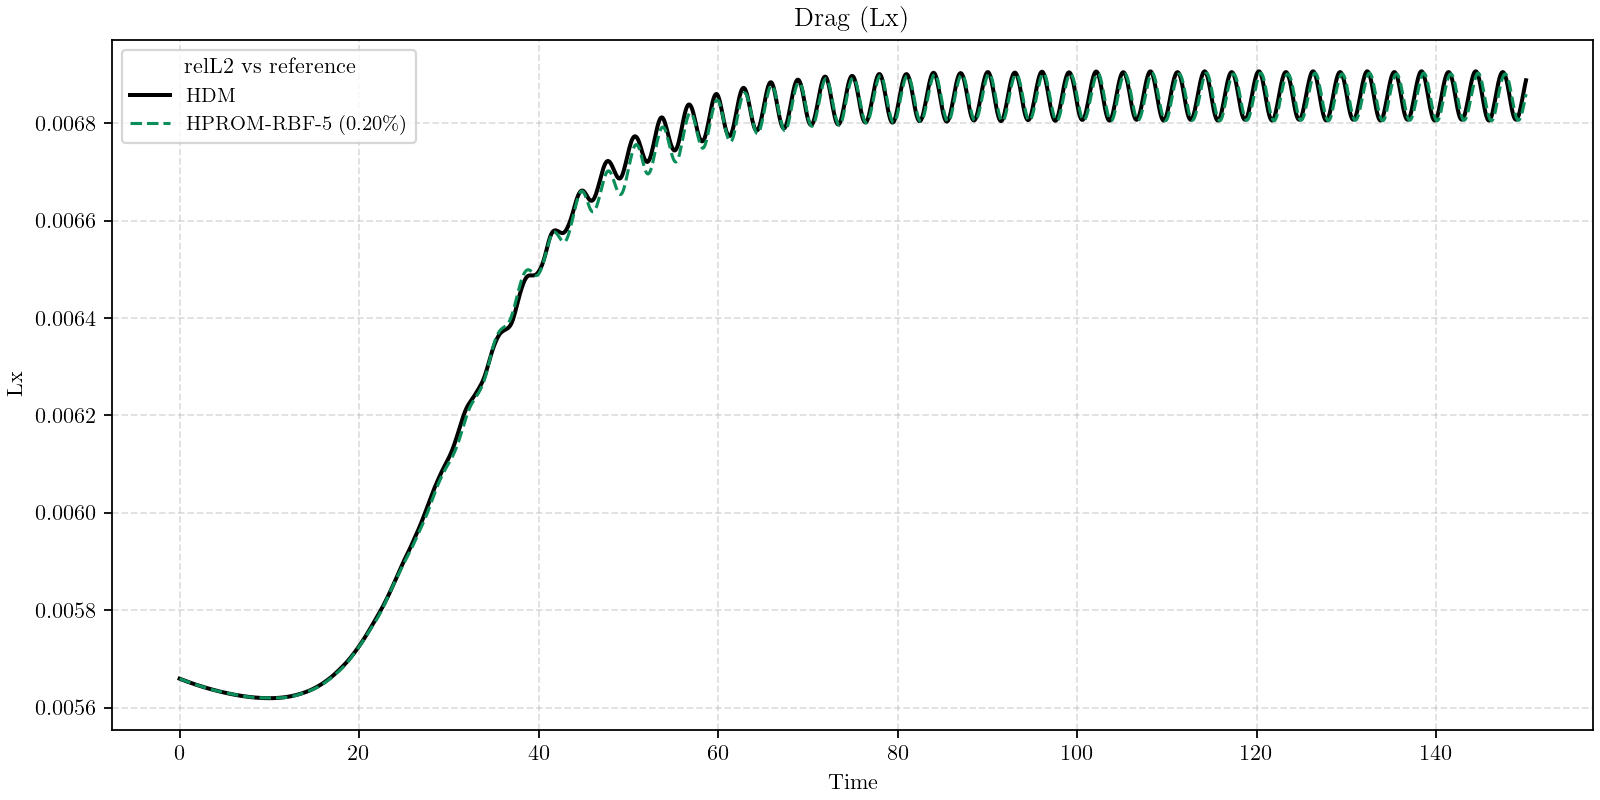
\includegraphics[width=0.92\textwidth]{Figures_AeroF/hprom_rbf_5_vs_hdm_drag_lx.png}
\end{frame}

\begin{frame}{Aero-F Cylinder: Local-HPROM-RBF ($N_c=3$) vs HDM (Drag $L_x$)}
\centering
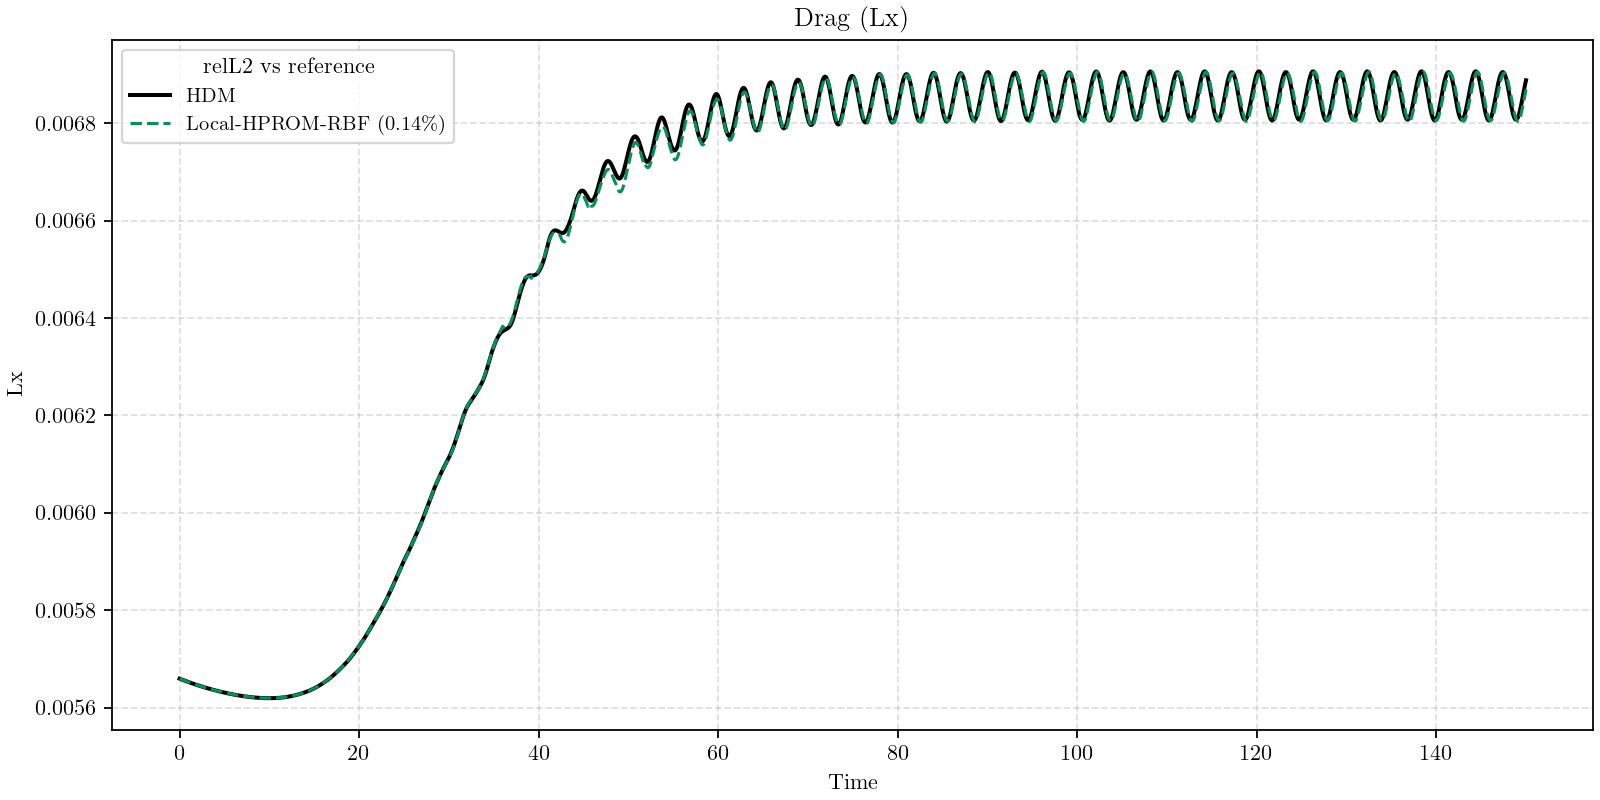
\includegraphics[width=0.92\textwidth]{Figures_AeroF/hprom_local_rbf_vs_hdm_drag_lx.png}
\end{frame}

\begin{frame}{Aero-F Cylinder: HPROM-GPR vs HDM (Drag $L_x$)}
\centering
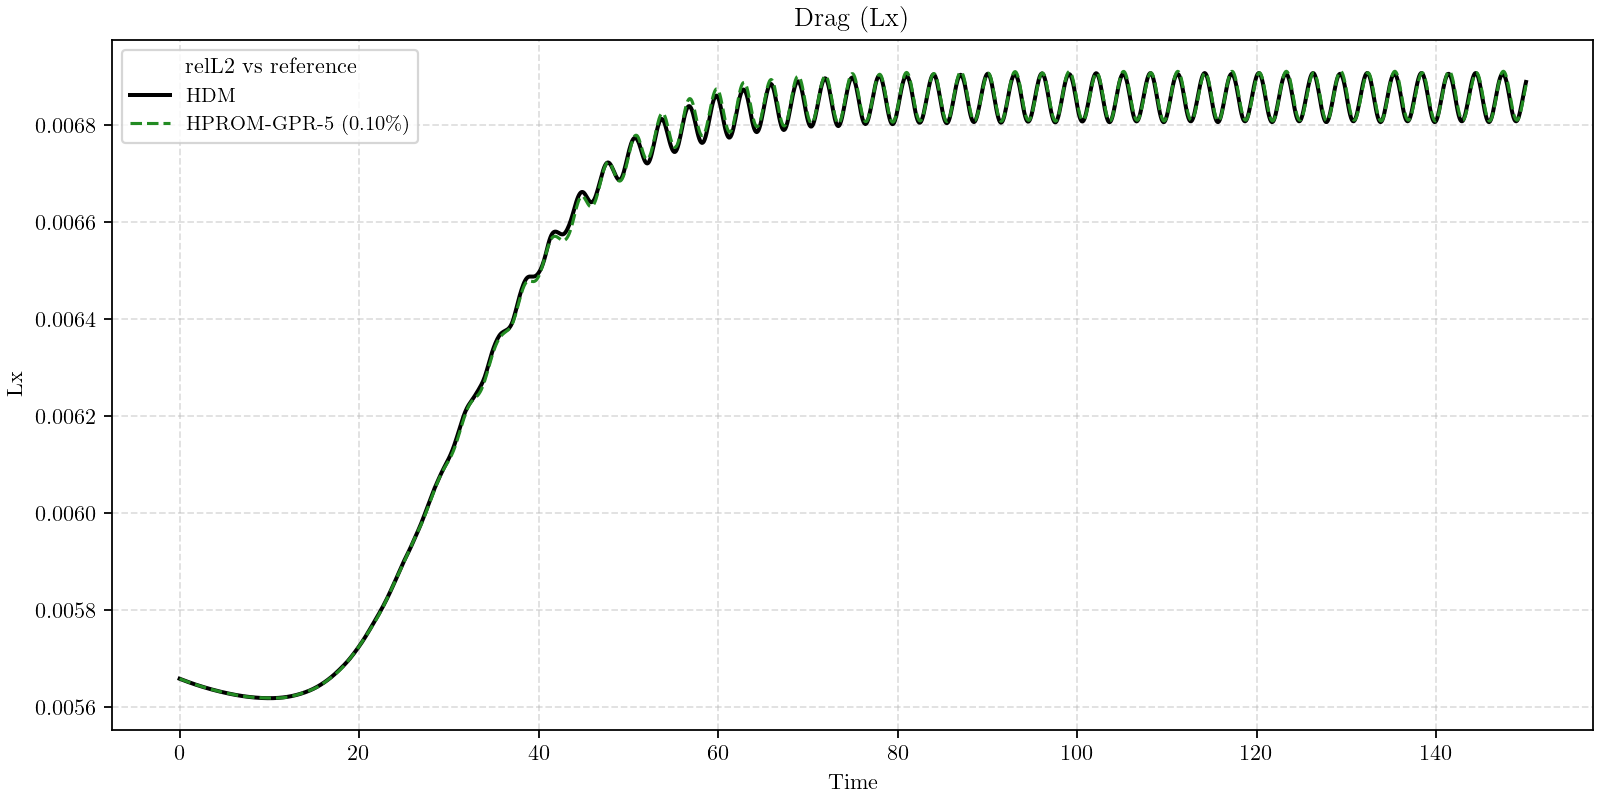
\includegraphics[width=0.92\textwidth]{Figures_AeroF/hprom_gpr_5_vs_hdm_drag_lx.png}
\end{frame}

\begin{frame}{Aero-F Cylinder: Local-HPROM-GPR ($N_c=3$) vs HDM (Drag $L_x$)}
\centering
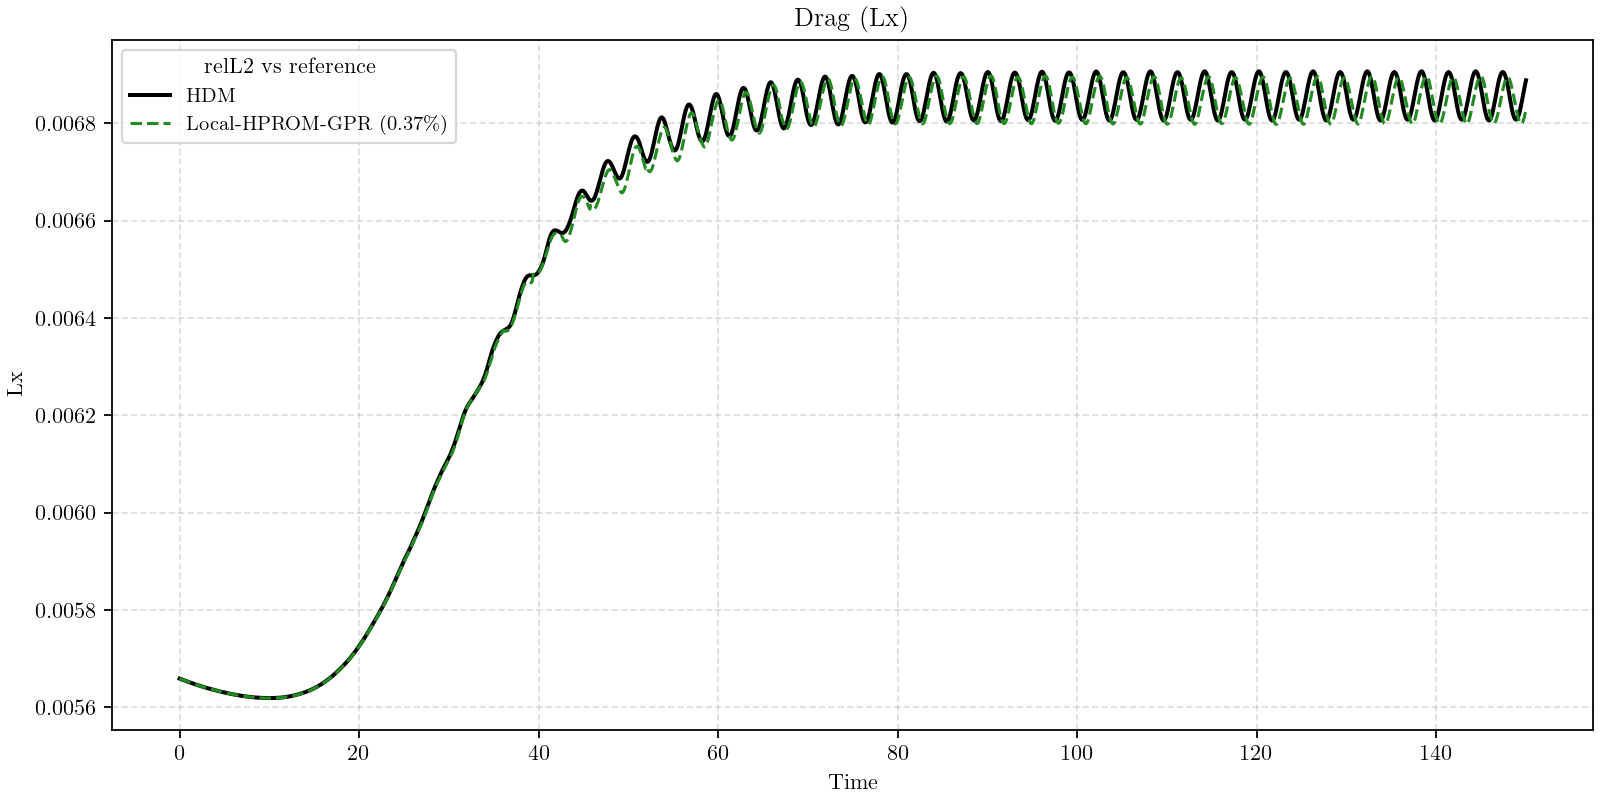
\includegraphics[width=0.92\textwidth]{Figures_AeroF/hprom_local_gpr_vs_hdm_drag_lx.png}
\end{frame}

\appendix

\begin{frame}{Appendix: Linear Selector Expansion}
\scriptsize
\[
\mathbf u^s=\mathbf u_{0,k^-}+\mathbf V_{k^-}\mathbf q_{k^-},
\qquad
k^+=\arg\min_{\ell}\|\mathbf u^s-\mathbf u_{c,\ell}\|_2^2.
\]
\[
\text{Let }\mathbf a_\ell:=\mathbf u_{0,k^-}-\mathbf u_{c,\ell},\quad
\mathbf b:=\mathbf V_{k^-}\mathbf q_{k^-}.
\]
\[
\|\mathbf u^s-\mathbf u_{c,\ell}\|_2^2
=\|\mathbf a_\ell+\mathbf b\|_2^2
=\|\mathbf a_\ell\|_2^2+\|\mathbf b\|_2^2+2\,\mathbf a_\ell^T\mathbf b.
\]
\[
\|\mathbf b\|_2^2=\|\mathbf V_{k^-}\mathbf q_{k^-}\|_2^2
\ \text{is independent of }\ell.
\]
\[
\Rightarrow\ 
k^+=\arg\min_{\ell}
\Big[
\|\mathbf u_{0,k^-}-\mathbf u_{c,\ell}\|_2^2
+2(\mathbf u_{0,k^-}-\mathbf u_{c,\ell})^T\mathbf V_{k^-}\mathbf q_{k^-}
\Big].
\]
Precompute
\[
\mathbf g_{k^-,\ell}:=\mathbf V_{k^-}^T(\mathbf u_{0,k^-}-\mathbf u_{c,\ell}),
\qquad
d_{k^-,\ell}:=\|\mathbf u_{0,k^-}-\mathbf u_{c,\ell}\|_2^2,
\]
which yields
\[
k^+=\arg\min_{\ell}\left(2\,\mathbf g_{k^-,\ell}^T\mathbf q_{k^-}+d_{k^-,\ell}\right).
\]
\end{frame}

\begin{frame}{Appendix: HQPROM Selector Expansion}
\scriptsize
\[
\mathbf u^s=\mathbf u_{0,k^-}+\mathbf V_{k^-}\mathbf q_{k^-}
+\mathbf H_{k^-}(\mathbf q_{k^-}\otimes\mathbf q_{k^-}).
\]
\[
\text{Let }\mathbf a_\ell:=\mathbf u_{0,k^-}-\mathbf u_{c,\ell},\quad
\mathbf b:=\mathbf V_{k^-}\mathbf q_{k^-},\quad
\mathbf c:=\mathbf H_{k^-}(\mathbf q_{k^-}\otimes\mathbf q_{k^-}).
\]
\[
k^+=\arg\min_{\ell}\|\mathbf u^s-\mathbf u_{c,\ell}\|_2^2
=
\arg\min_{\ell}
\|\mathbf a_\ell+\mathbf b+\mathbf c\|_2^2.
\]
\[
\|\mathbf a_\ell+\mathbf b+\mathbf c\|_2^2
=\|\mathbf a_\ell\|_2^2+\|\mathbf b\|_2^2+\|\mathbf c\|_2^2
+2\,\mathbf a_\ell^T\mathbf b
+2\,\mathbf a_\ell^T\mathbf c
+2\,\mathbf b^T\mathbf c.
\]
\[
\|\mathbf b\|_2^2,\ \|\mathbf c\|_2^2,\ 2\,\mathbf b^T\mathbf c
\ \text{are independent of }\ell.
\]
\[
\Rightarrow\ 
k^+=\arg\min_{\ell}
\Big[
\|\mathbf u_{0,k^-}-\mathbf u_{c,\ell}\|_2^2
\]
\[
\quad
+2(\mathbf u_{0,k^-}-\mathbf u_{c,\ell})^T\mathbf V_{k^-}\mathbf q_{k^-}
+2(\mathbf u_{0,k^-}-\mathbf u_{c,\ell})^T\mathbf H_{k^-}(\mathbf q_{k^-}\otimes\mathbf q_{k^-})
\Big].
\]
Define
\[
\mathbf m_{k^-,\ell}^T(\mathbf q\otimes\mathbf q)
:=
(\mathbf u_{0,k^-}-\mathbf u_{c,\ell})^T\mathbf H_{k^-}(\mathbf q\otimes\mathbf q),
\]
then
\[
k^+=\arg\min_{\ell}
\left(
2\,\mathbf g_{k^-,\ell}^T\mathbf q_{k^-}
+2\,\mathbf m_{k^-,\ell}^T(\mathbf q_{k^-}\otimes\mathbf q_{k^-})
+d_{k^-,\ell}
\right).
\]
\end{frame}

\begin{frame}{Appendix: HPROM-GPR Selector Expansion}
\scriptsize
\[
\mathbf u^s=
\mathbf u_{0,k^-}
+\mathbf V_{k^-}\mathbf q_{k^-}
+\bar{\mathbf V}_{k^-}\bar{\mathbf q}_{k^-},
\qquad
\bar{\mathbf q}_{k^-}=\mathcal N_{\mathrm{GPR},k^-}(\mathbf q_{k^-}).
\]
\[
\text{Let }\mathbf a_\ell:=\mathbf u_{0,k^-}-\mathbf u_{c,\ell},\quad
\mathbf b:=\mathbf V_{k^-}\mathbf q_{k^-},\quad
\mathbf c:=\bar{\mathbf V}_{k^-}\bar{\mathbf q}_{k^-}.
\]
\[
\|\mathbf u^s-\mathbf u_{c,\ell}\|_2^2
=\|\mathbf a_\ell+\mathbf b+\mathbf c\|_2^2
\]
\[
\ =\ \|\mathbf a_\ell\|_2^2+\|\mathbf b\|_2^2+\|\mathbf c\|_2^2
+2\,\mathbf a_\ell^T\mathbf b
+2\,\mathbf a_\ell^T\mathbf c
+2\,\mathbf b^T\mathbf c.
\]
\[
\|\mathbf b\|_2^2,\ \|\mathbf c\|_2^2,\ 2\,\mathbf b^T\mathbf c
\ \text{are independent of }\ell.
\]
\[
\Rightarrow\ 
k^+=\arg\min_{\ell}
\Big[
\|\mathbf u_{0,k^-}-\mathbf u_{c,\ell}\|_2^2
+2(\mathbf u_{0,k^-}-\mathbf u_{c,\ell})^T\mathbf V_{k^-}\mathbf q_{k^-}
+2(\mathbf u_{0,k^-}-\mathbf u_{c,\ell})^T\bar{\mathbf V}_{k^-}\bar{\mathbf q}_{k^-}
\Big].
\]
Hence, with
\[
\bar{\mathbf g}_{k^-,\ell}:=\bar{\mathbf V}_{k^-}^T(\mathbf u_{0,k^-}-\mathbf u_{c,\ell}),
\]
\[
k^+=\arg\min_{\ell}
\left(
2\,\mathbf g_{k^-,\ell}^T\mathbf q_{k^-}
+2\,\bar{\mathbf g}_{k^-,\ell}^T\bar{\mathbf q}_{k^-}
+d_{k^-,\ell}
\right).
\]
\end{frame}

\end{document}
